\documentclass{standalone}
\usepackage{xr-hyper}
\usepackage{hyperref}
\externaldocument[C3-]{Chapter3}
\begin{document}
\chapter{Data Analysis}
\label{Data Analysis}
As discussed in Chapter\ref{C3-Inertial Measurement Unit} in the Error section(\ref{C3-Error} on page \pageref{C3-Error}). IMU, during measurement suffer from accumulated error.\pageref{C3-Error}\\
The measurement along the pathway of road surface consists of a sampling of measurements at specific time intervals (usually in the order of milliseconds).So the road profile can be seen as an electronically acquired digital signal and consequently it is necessary clean up the signal from the noise\footnote{An unknown modifications that a signal may suffer during capture}, it may also be useful to delete certain information in the signal that is not of interest, or correct it from the drift (\ref{C3-Error}).\\


\noindent This cleaning procedure, also called filtering,it is used in the theory of signal analysis.
It is an essential aspect in the evaluation of the profile, \cite{little_book}. In brief, a digital filter represents a procedure that transforms a series of numbers into a new series of numbers, \cite{little_book}.\\
From the measurement obtained by the sensors, particular attention is given to the vertical acceleration signal and to the rotation vectors. \\
The rotation vectors will be useful for reorienting the signals obtained from the smartphone\cite{Andro} respect to the vehicle axes, while the vertical acceleration signal will be subject to various filtering operations depending on the final index to be obtained.\\\\
First of all, it is necessary to pay some attention to some dynamics\footnote{branch of mechanics that deals with the study of the motion of bodies and their causes or, more concretely, of the circumstances that determine and modify it} physical principles , about the operations that can be done, on the acceleration signal to get the position and vice-versa.\\\\
Given a position versus time of an object, $x(t)$, the velocity, $v(t)$, can be found by taking the first derivative.\\
\begin{center}
{\large $v(t) = \dfrac{dx}{dt}$}
\end{center}
Acceleration, $a(t)$, can be found by taking the second derivative of position or first
derivative of velocity.
\begin{center}
{\large $a(t) = \dfrac{d^{2}x}{dt^{2}} = \dfrac{dv}{dt}$}
\end{center}
However, is interesting to reverse this process and find the position signal given an acceleration signal. To do that, a double integration must be performed on the acceleration signal.
In principle, using double integration on an acceleration signal to get a position signal, the initial position and initial velocity must be known. After the first integration, the initial velocity should be added to the result, as the initial position should be added after the second integration. These operations are illustrated in the following equations
\begin{center}
\begin{equation}
 {\large v(t) = v(t_{0}) + \int_{t_{0}}^{t} \! a(\tau) \, \mathrm{d}\tau}
\end{equation}

Where: \\
\begin{table}[ht]
\centering
    \begin{tabular}{ | l | l |}
    
    \hline
    Symbol & Description \\ \hline
   \quad  $t_{0}$ & Initial Time \\ \hline
	   \quad  $v(t_{0})$ & Initial Velocity\\  
\hline 
    \end{tabular}
\end{table}
\end{center}

\noindent To get the position signal from velocity, is used the followed formula:
\begin{center}
\begin{equation}
 {\large x(t) = x(t_{0}) + \int_{t_{0}}^{t} \! v(\tau) \, \mathrm{d}\tau.}
\end{equation}

Where: \\
\begin{table}[ht]
\centering
    \begin{tabular}{ | l | l |}
    
    \hline
    Symbol & Description \\ \hline
   \quad  $t_{0}$ & Initial Time \\ \hline
	   \quad  $x(t_{0})$ & Initial Position \\  
\hline 
    \end{tabular}
\end{table}
\end{center}
\noindent Therefore, for a double integration of the acceleration, the two initial
conditions (velocity and position) must be known to avoid integration errors. However,
the only way to get these initial conditions is through direct measurement, which is often
impractical or unobtainable. By  data filtering, it is developed an approach that does not require knowledge of initial conditions.\\
To perform a numerical integration it is necessary to choose one integration algorithm of the many existing. 
The acceleration signal is sampled, making it a discrete function of time having a sampling frequency, $f_{s}$, associated with it. The easiest way to perform numerical integration is to use the rectangular integration method. This method uses an accumulator to sum all past sampled inputs and the current input sample and divide by the sampling rate. Rectangular integration is represented by the following difference equation:

\begin{center}
$y(n) = \dfrac{1}{f_{s}} \sum_{k=0}^{n} x(n-k) = y(n-1) + \dfrac{1}{f_{s}} x(n)$
\end{center}

\noindent Another numerical integration method uses the trapezoidal rule. 
The results are more precise with this method than the rectangular method. The difference equation for trapezoidal integration is:

\begin{center}
$y(n) = y(n-1) + \dfrac{1}{2 f_{s}}[x(n-1) + x(n)], n > 0$
\end{center}

The figure below show the difference using both methods.

\vspace{0.35cm}
\begin{figure}[ht]
\centering
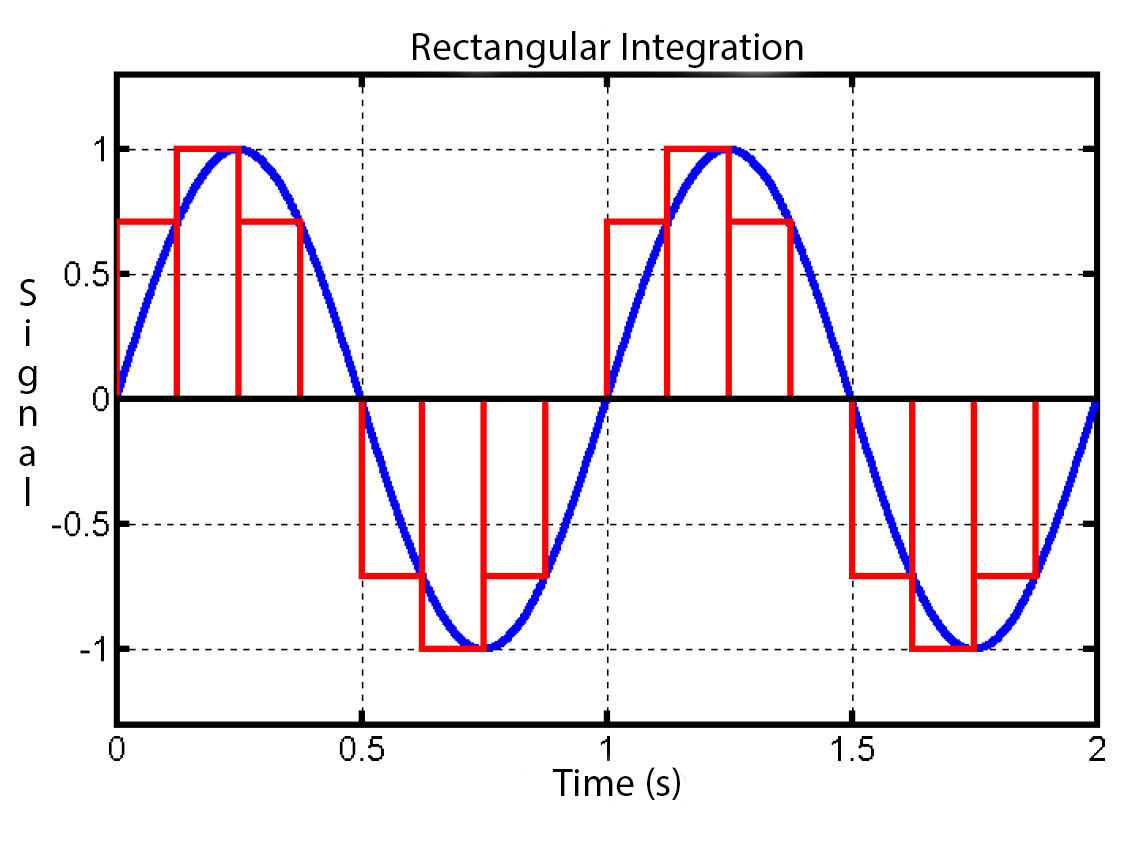
\includegraphics[scale=0.55]{RectangularInte}
\hspace{0.5cm}
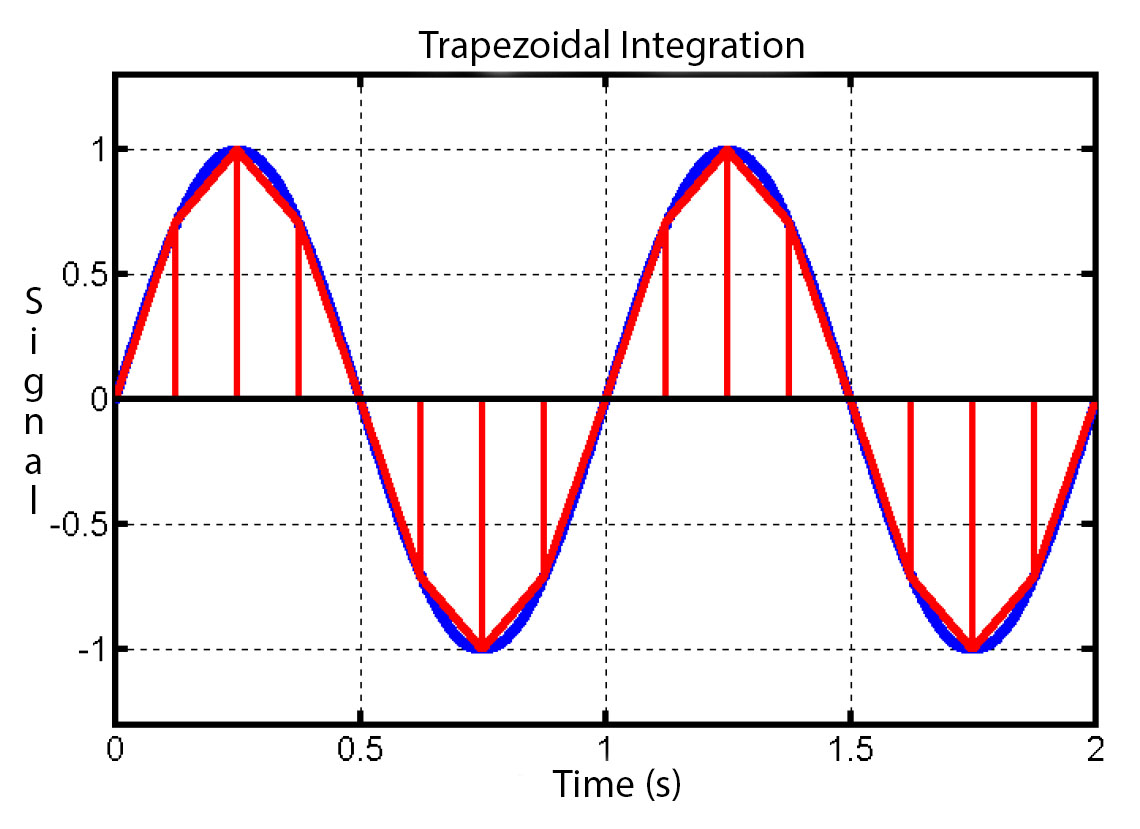
\includegraphics[scale=0.55]{TrapezoidalIntegration}
\caption{Integration using Rectangular (left) and Trapezoidal (right) methods of Sine Wave.}
\label{fig:Rectangular and Trapezoidal Integration}
\end{figure}

\noindent The integration was carried out using the trapezoidal method by the MATLAB suite. But without adequate cleaning of the signal, the result presents very error, caused by the drift and noise. \\
Various signal cleanup procedures will be discussed. The figure below shows the result of a raw signal integration using trapezoidal method.

\begin{figure}
  \centering
  \subfloat[Acceleration]{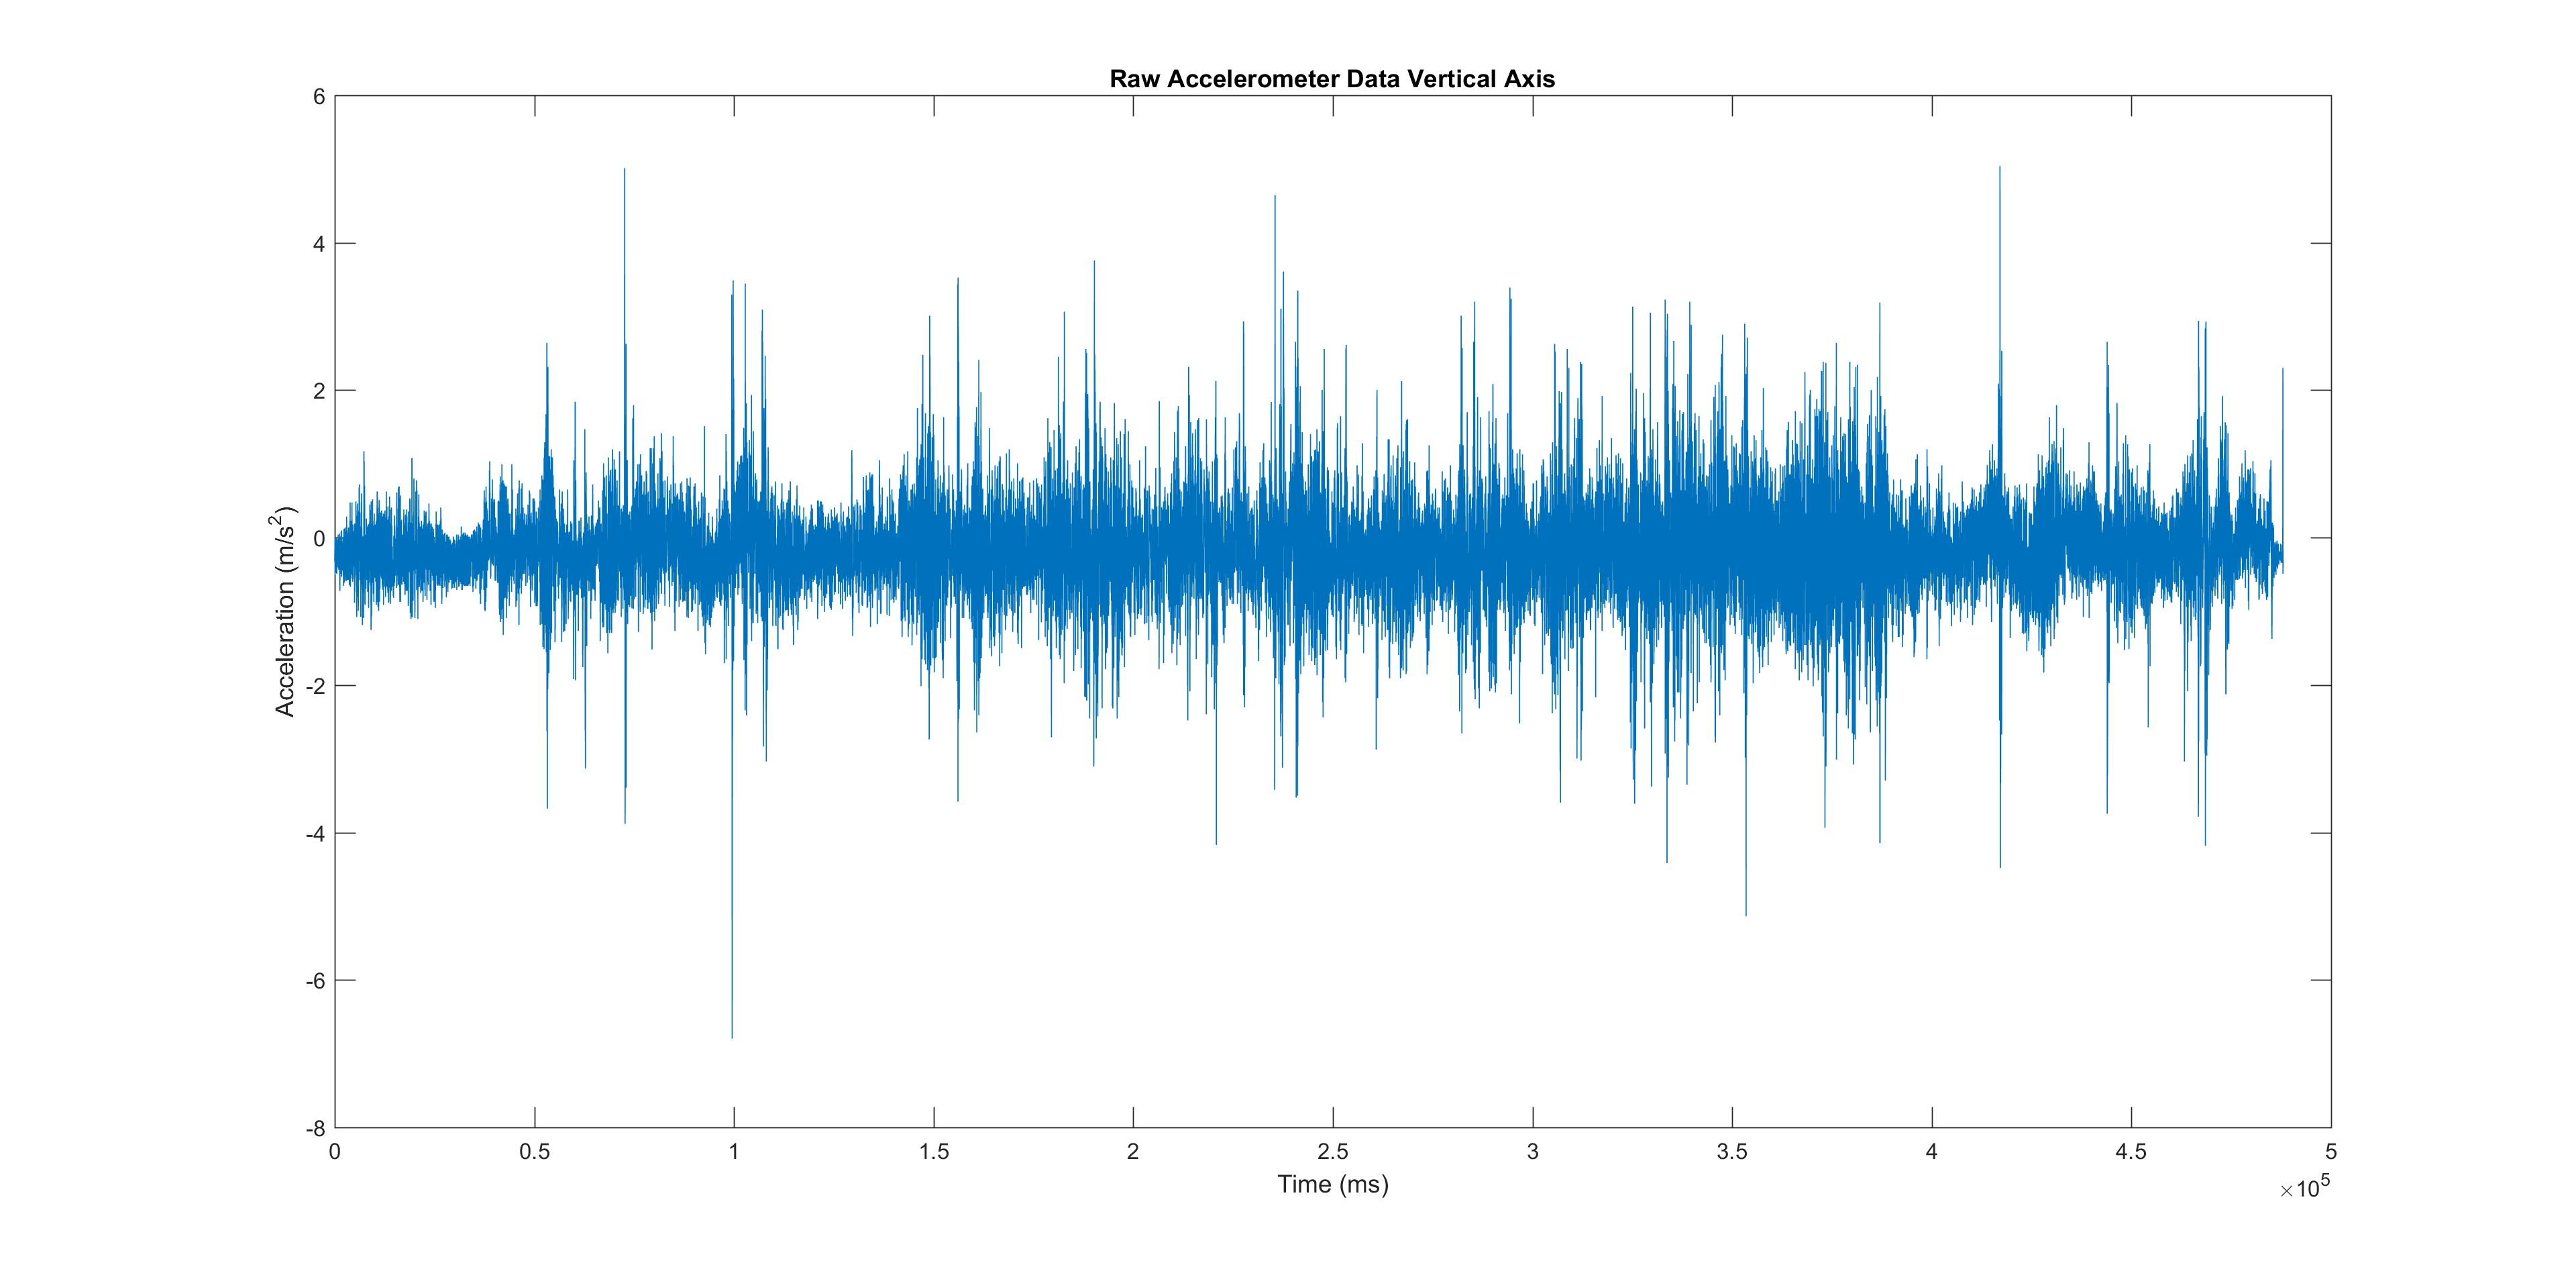
\includegraphics[scale=0.11]{RawAccelerometer}\label{fig:Raw Accelerometer}}  
  
  \subfloat[Velocity]{\includegraphics[scale=0.11]{VelocityIntegration}\label{fig:Velocity}}

  \subfloat[Displacement]{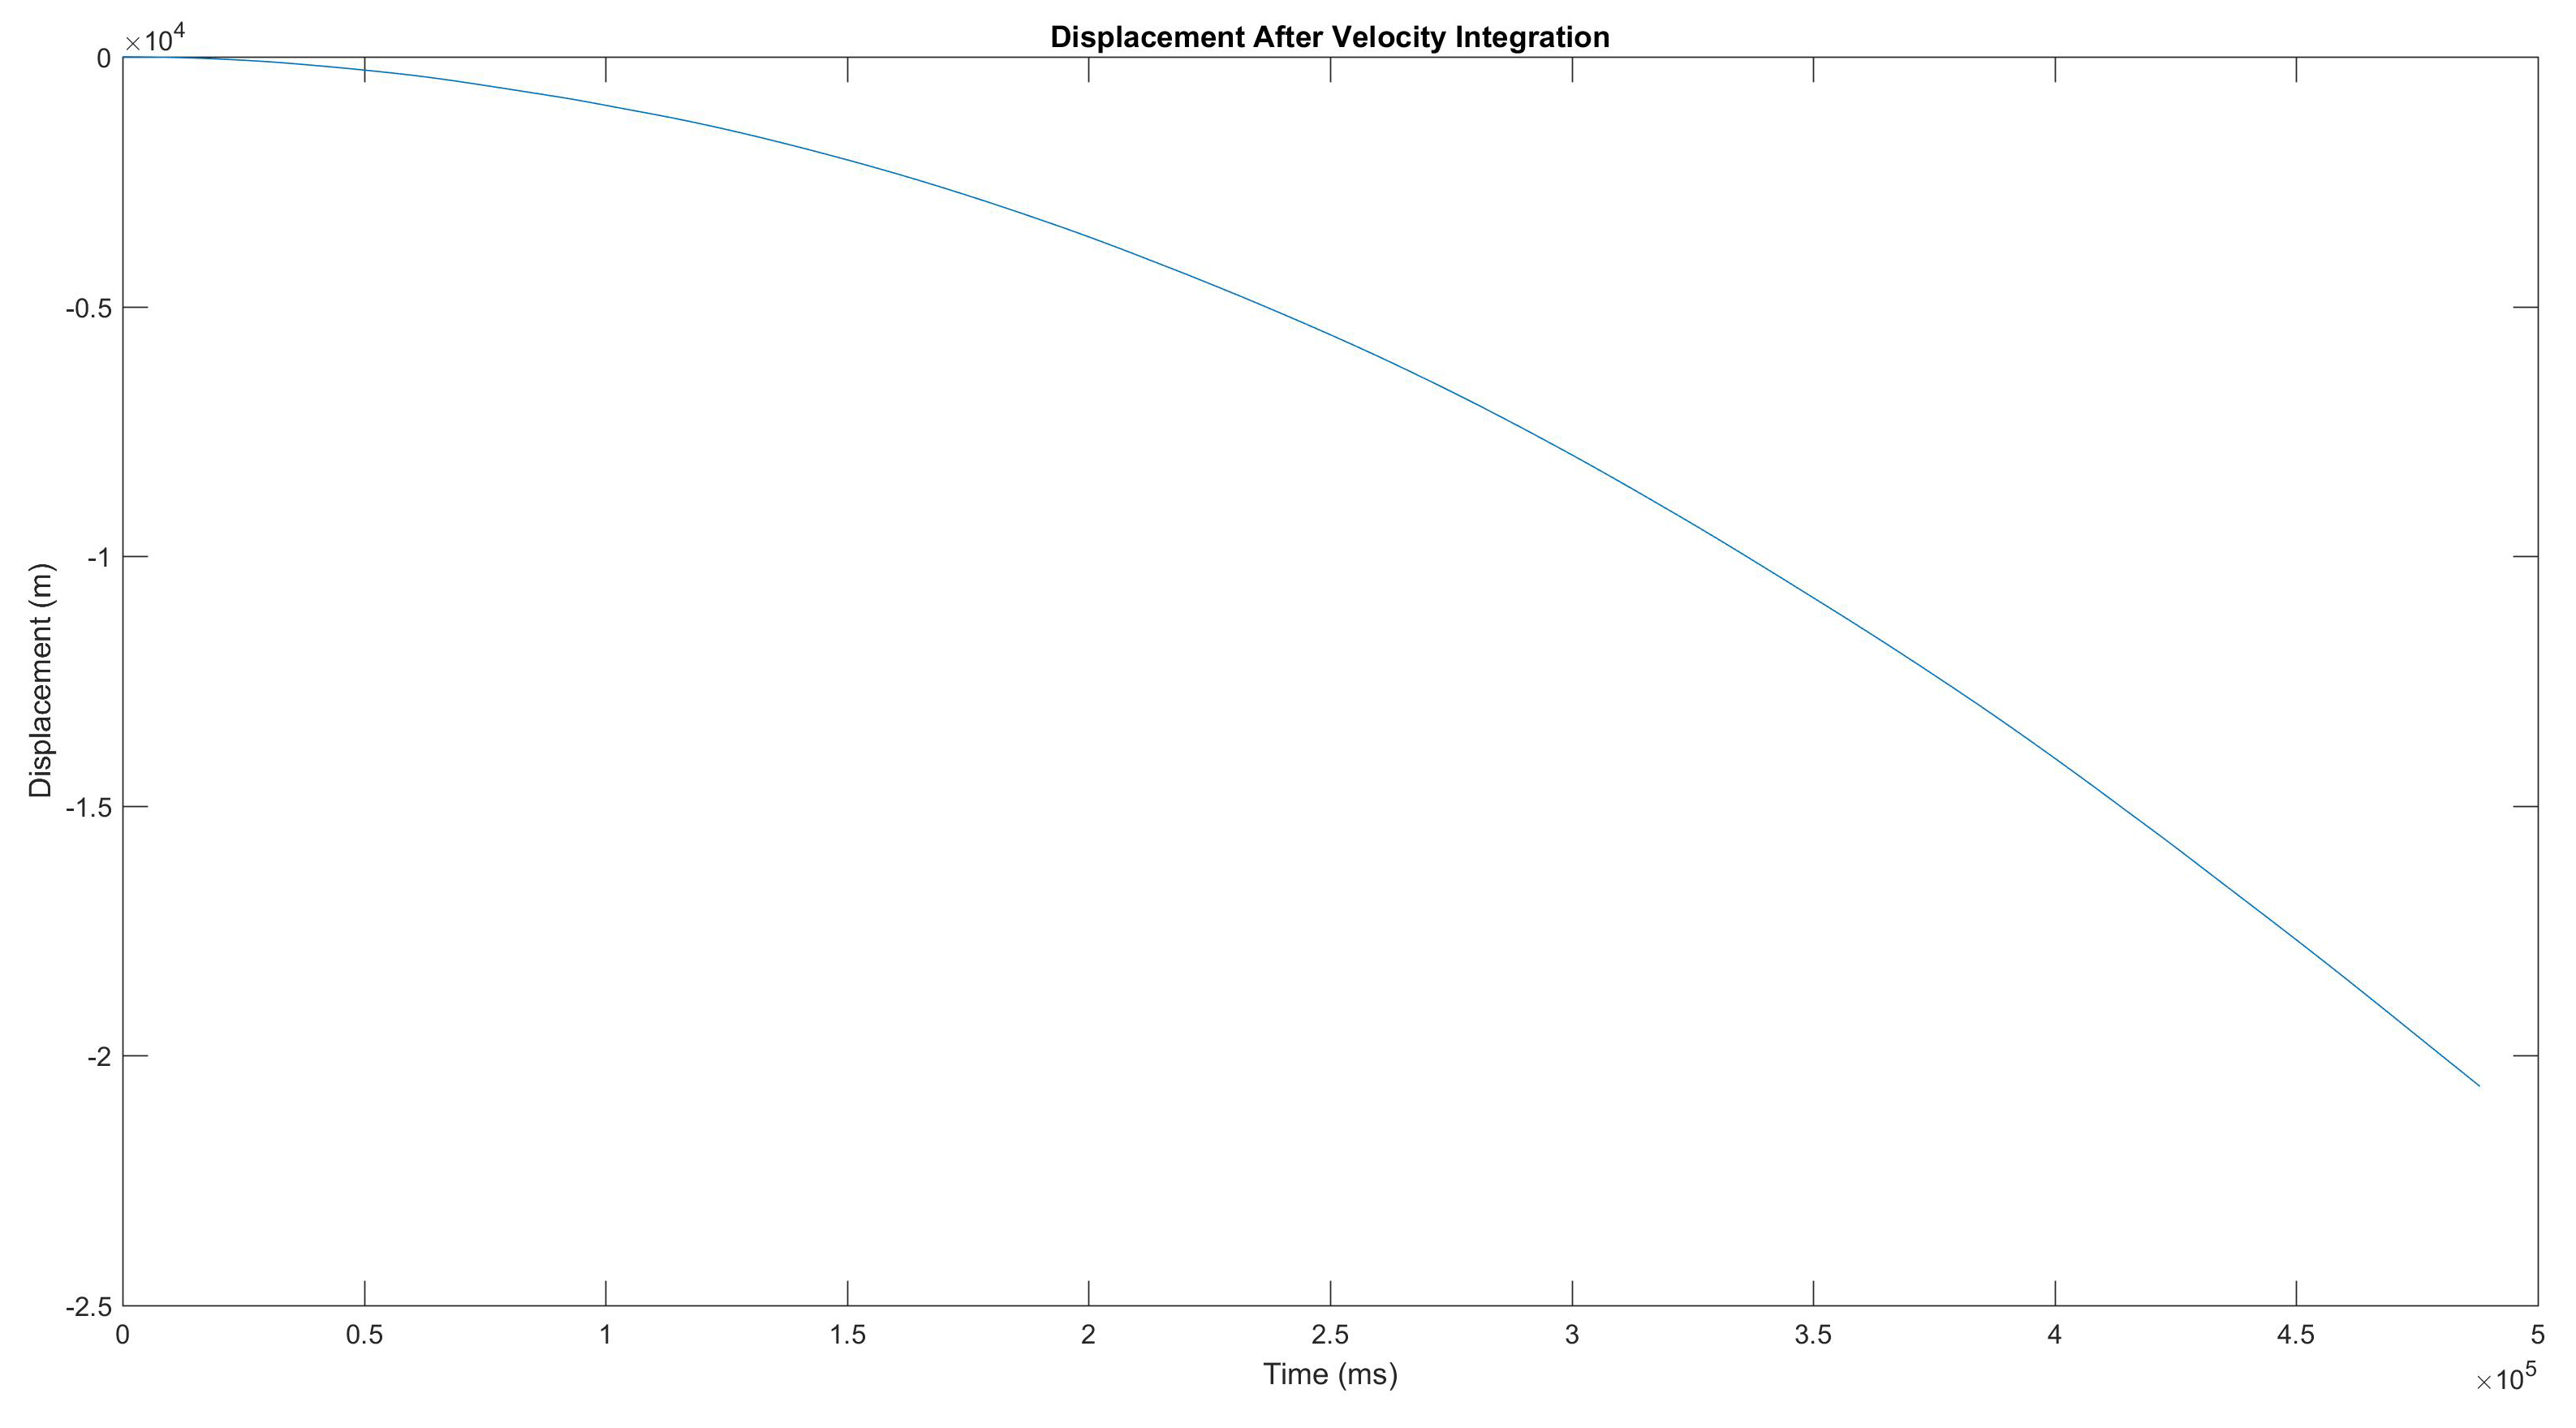
\includegraphics[scale=0.11]{DisplacementIntegration}\label{fig:Displacement}}  
  \caption{The result of double integration of a Raw Signal}
  \label{fig:Integration of Raw Data}
\end{figure}
\clearpage

\noindent As is possible see, the result is not realistic, considering it is vertical acceleration, so it is necessary to perform various steps to fix and clean the signal. First of all, the signal reorientation will be carried out respect the axes of the vehicle, and subsequently, various filter operations to clean the signal.

\section{Accelerometer Reorientation} \label{Accelerometer Reorientation}
\noindent The Cartesian reference system of the phone must be aligned with the vehicle reference system, to detect the vehicle motion correctly.
As shown in the figure below.

\begin{figure}[ht]
  \centering
  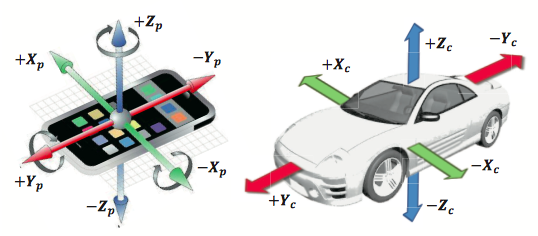
\includegraphics[scale=0.7]{phonecarorientation}  
  \caption{Correct alignment of smartphone respect to the vehicle cartesian frame.}
  \label{fig:Smartphone cartesian frame alignment respect Car axis.}
\end{figure}
\noindent Smartphone accelerometer detects the following accelerations: $a_{x_{p}}$ , $a_{y_{p}}$ and $a_{z_{p}}$ . To determine the accelerations felt by the vehicle and locate road surface anomalies. The accelerometer must detect what happens in the direction perpendicular ($Z$ axes) to the vehicle \cite{mohan2008nericell}.
Respectively the $X_{p}$ axis identifies the longitudinal direction, $Y_{p}$ axis the transverse direction and $Z_{p}$ the perpendicular direction respect to the $xy$ plane.

\noindent To detect road anomalies, the direction of the z-axis must correspond to the direction of the z axis. If this condition subsists, the accelerometer is well oriented, contrarily it is not well oriented and needs to be reoriented. But even if starting from a precise orientation condition, during travel the phone may be moving, or due to unexpected vehicle movements, travel of climbing, downhill, curve, all of these causes could affect the misalignment of the smartphone frame respect to the vehicle frame.

\noindent The reorientation can be performed by the Euler Angles. Three angles that allow to defining the orientation in space of any body through a succession of elementary rotations.\cite{diebel2006representing}
The $XYZ$ sequence was defined,a rotation around the $x$ axis by an angle $\alpha$ (roll angle), one around the $y$ axis by $\beta$ (pitch angle) and one around the $z$ axis by  $\gamma$ (yaw angle).\\\\
\noindent The equations that allows to reoriented data by the $\alpha$, $\beta$, $\gamma$, angle are:\cite{Andro}
\begin{equation}
a_{x_{reor}} = \cos (\beta) a_{x_{p}} + \sin (\beta) \sin (\alpha) a_{y_{p}} + \cos (\alpha) \sin (\beta) a_{z_{p}} 
\end{equation}
\begin{equation}
a_{y_{reor}} = \cos (\alpha) a_{y_{p}} - \sin (\alpha) a_{z_{p}}
\end{equation}
\begin{equation}
a_{z_{reor}} = -\sin (\beta) a_{x_{p}} + \cos (\beta) \sin (\alpha) a_{y_{p}} + \cos (\beta) \cos (\alpha) a_{z_{p}}
\end{equation}


\noindent The figure below, show an example of reoriented data.
\begin{figure}[ht]
  \centering
  \subfloat[Raw]{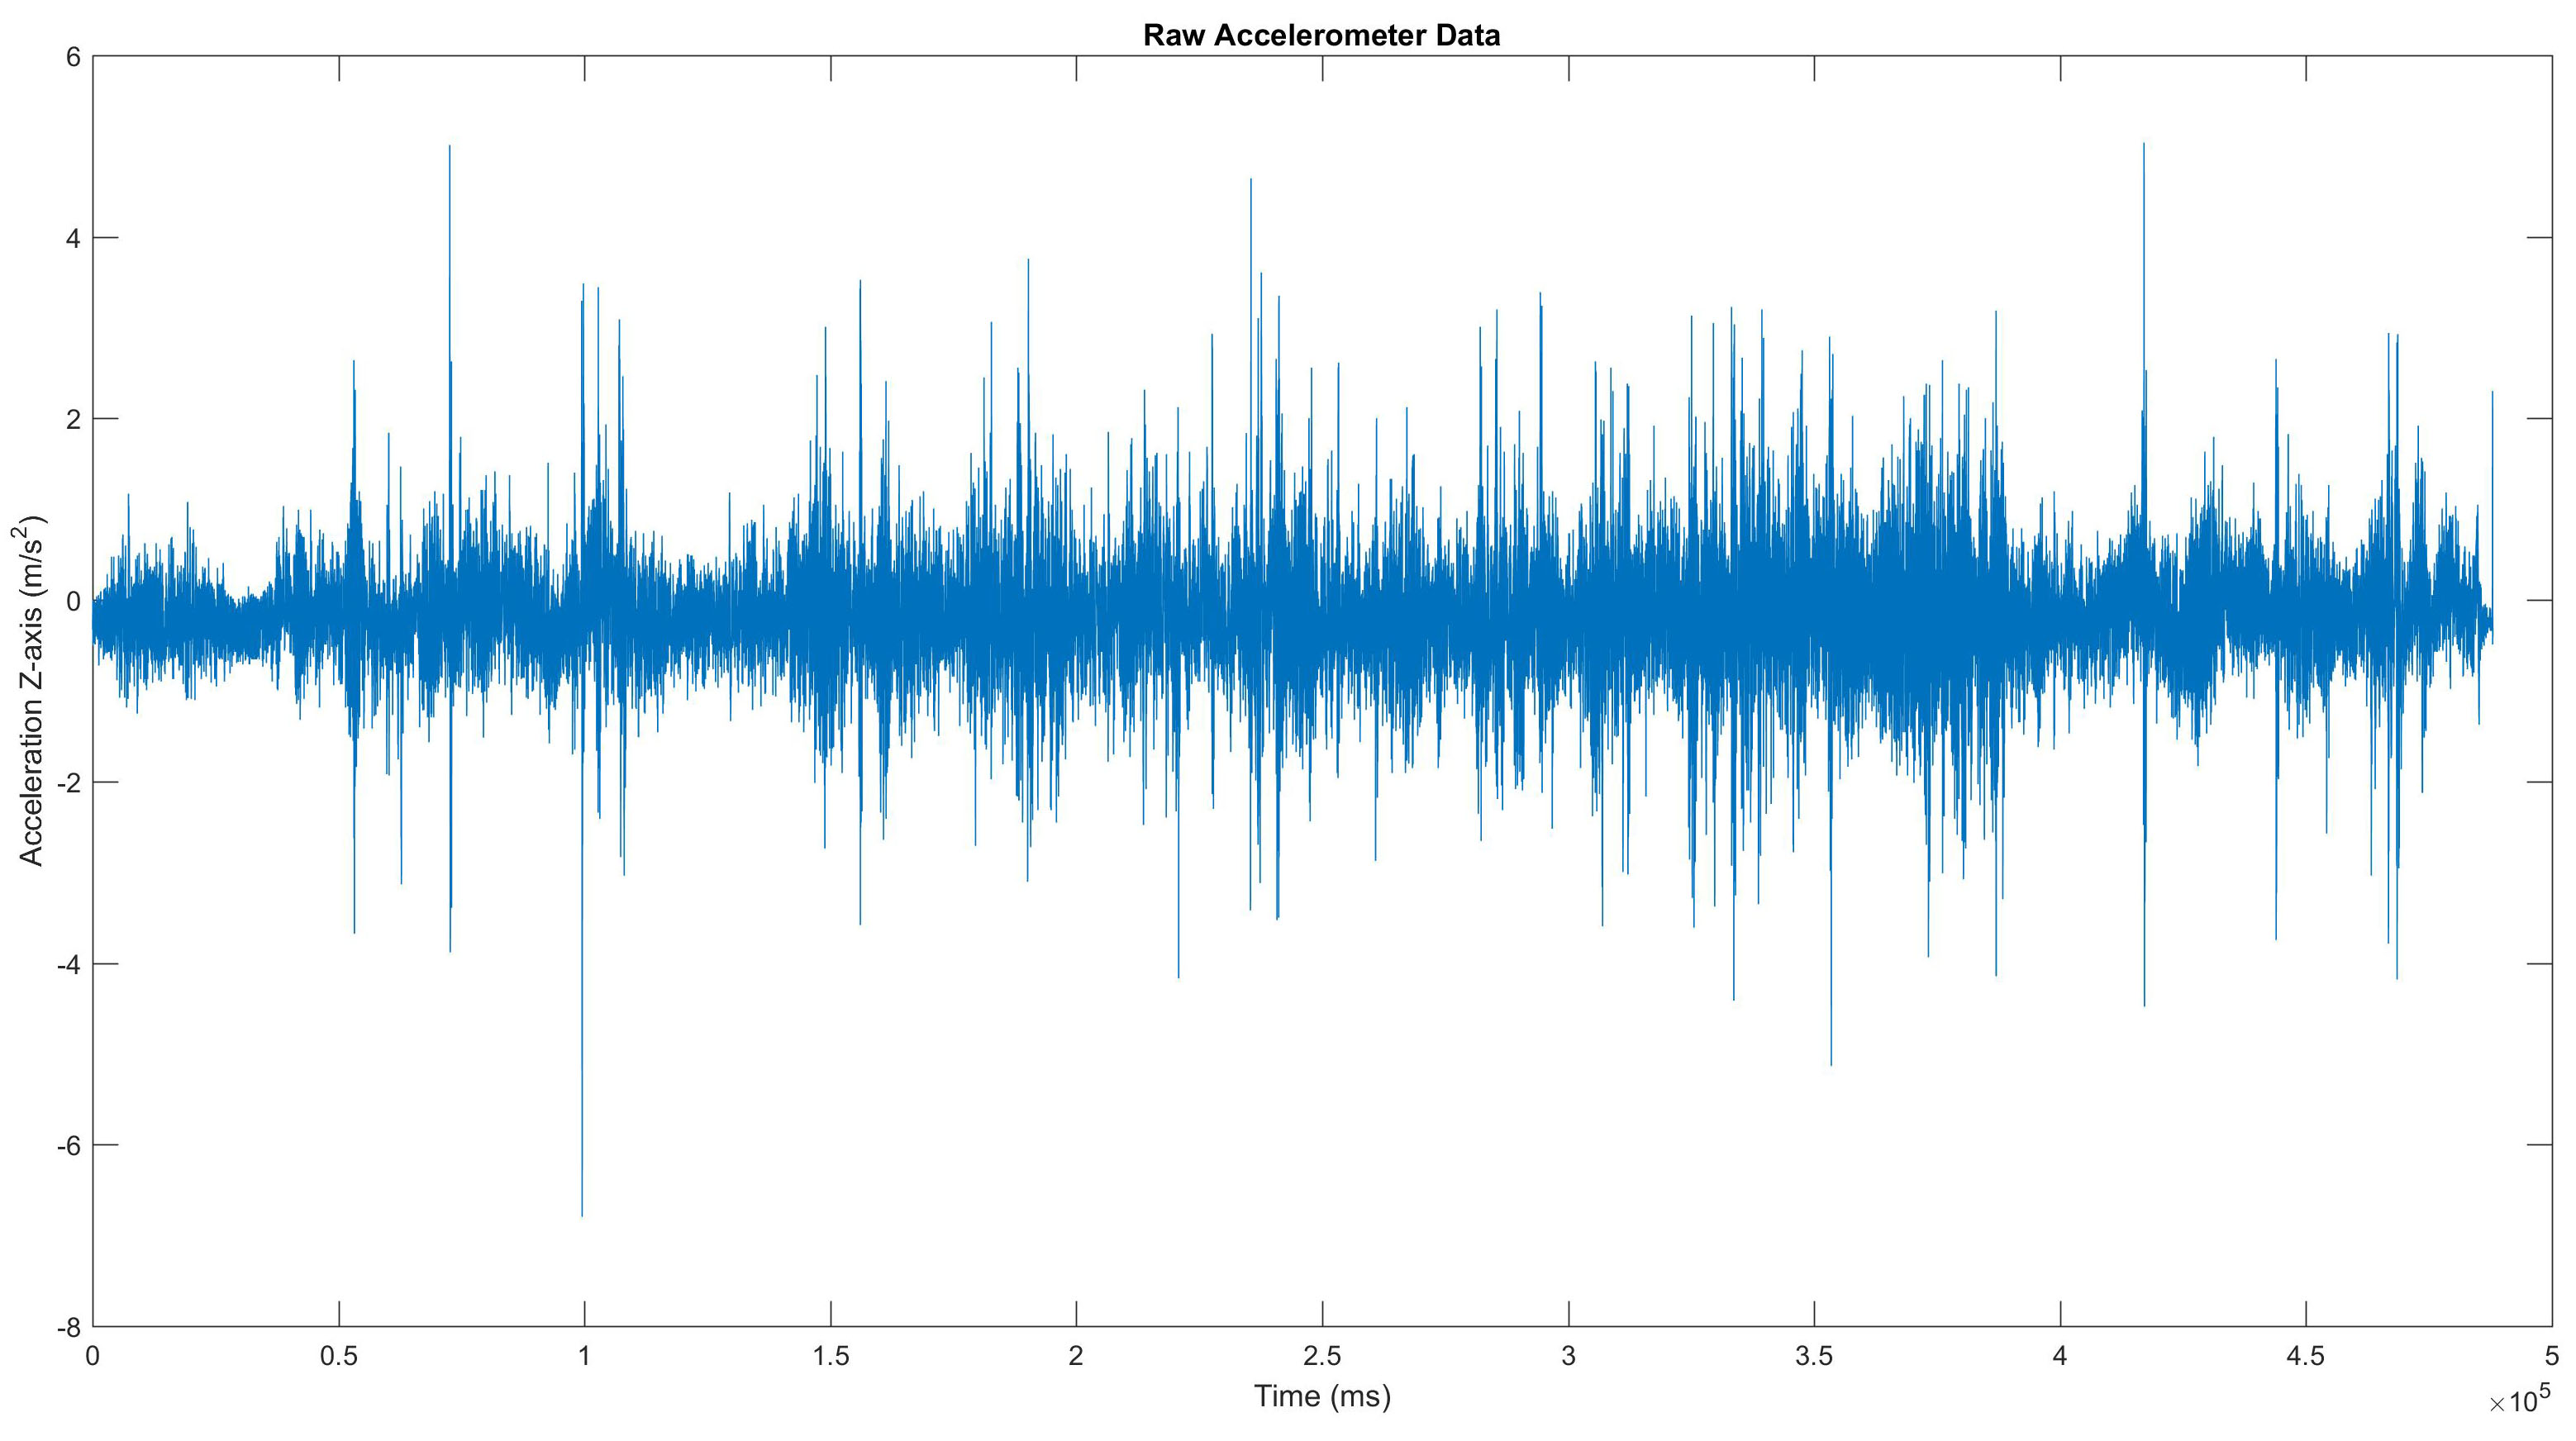
\includegraphics[scale=0.11]{raw}\label{fig:Raw Accelerometers}}  
  
  \subfloat[Reoriented]{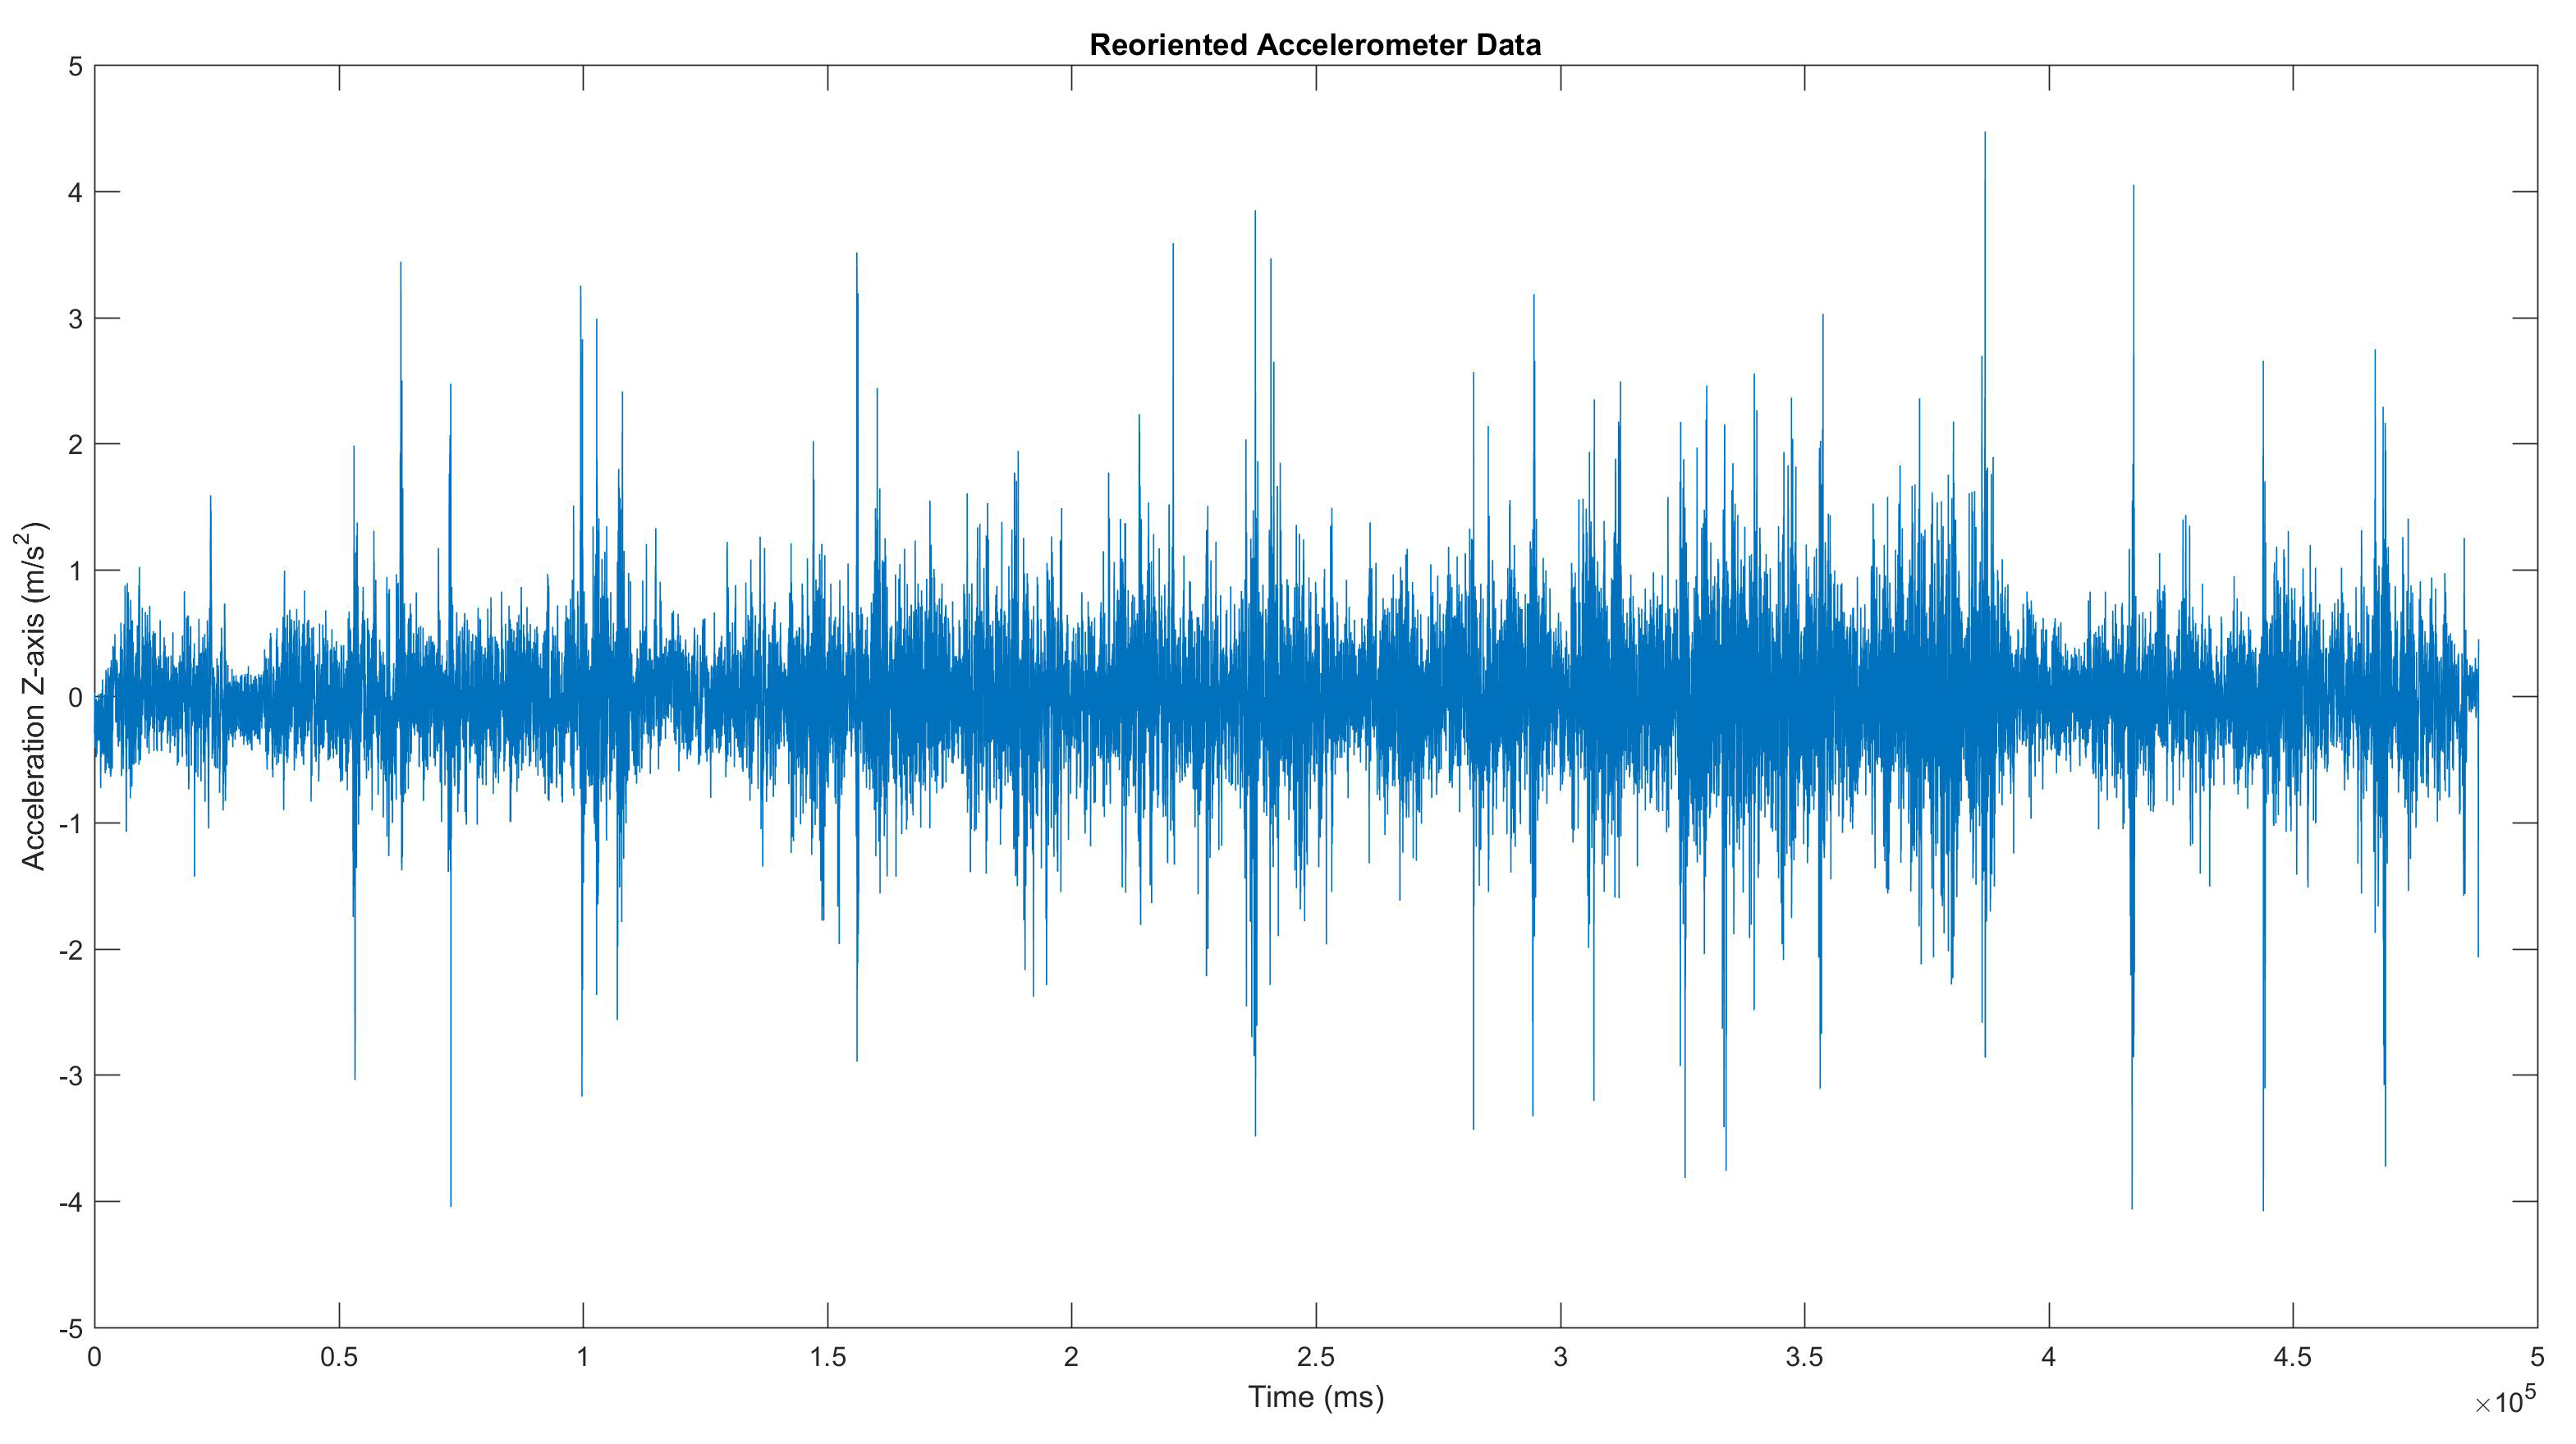
\includegraphics[scale=0.11]{reoriented}\label{fig:Reoriented Accelerometer}}

 
  \caption{The result of reorientation of raw data}
  \label{fig:Accelerometer Reoriented}
\end{figure}

\section{Data Filtering} \label{Data Filtering}
As can be seen in the figure \ref{fig:Integration of Raw Data}, a data filtering operation is needed to clear the signal and perform better integration.
It is necessary to apply:

\begin{itemize}
\item A series of preliminary filters for removing unimportant information.
\item A digital filter for removing certain frequency components that cause the error at the stage of integration.
\end{itemize}



\subsection{Preliminary Filtering}\label{Preliminary Filtering}
During signal capture, it is important to consider some information that can be removed, since they are not relevant to the final calculation.\\
These principally regard:
\begin{itemize}
\item The background noise generated by engine vibrations.
\item Acceleration components recorded at the moment the vehicle is stationary, so when its velocity is equal to $0$ $\si{\km\per\hour}$.
\end{itemize}

\noindent These two filters are applied to all three indexes (IRI, Critical Points, Simple Acceleration Points) that are extrapolated from the data series.

\subsubsection{Remove Engine Vibrations Filter} \label{Remove Engine Vibrations Filter}
Considering the vehicle in a stationary position, both flat, uphill and downhill, with no any external form of acceleration given by the pilot, so at no speed. Many measurements have been made to see how much the engine vibration affects the process of data acquisition.\\\\
Analyzing these measurements, two thresholds, one minimum and one maximum were identified, called respectively \textbf{$a_{min_{th}}$} and \textbf{$a_{max_{th}}$}.\\\\
Next, considering the generic acceleration signal at time $a_{t}$, the data series is thus modified:


\begin{center}
\[
    \left\{
                \begin{array}{ll}
                  a_{t} = a_{t} - a_{max_{th}}; \quad 	if \quad a_{t} > a_{max_{th}}\\
              	  a_{t} = a_{t} + |a_{min{th}}|; \quad  if \quad a_{t} < a_{min_{th}}
                \end{array}
              \right.
\]
\end{center}
\clearpage
\noindent Or:

\begin{center}
$a_{t} = \sqrt{\dfrac{1}{k} (a_{t_{i}}^{2} + a_{t_{i+1}}^{2} + ... + a_{t_{i+k}}^{2} )} $\\
\end{center}
\begin{center}
$if\quad  a_{min_{th}} <= a_{t} <= a_{max_{th}} $


Where $k$ is the number of a predefined window, and all the values that falls into the window indexes will be considered.\\ 
So the final value $a_{t}$ will be calculated as the Root Mean Square of that values.
\end{center}

\noindent The figure below shows an example of applying the filter to a series of data subject only to the reorientation operation\ref{Accelerometer Reorientation}.

\begin{figure}[H]	

\subfloat[Acceleration]{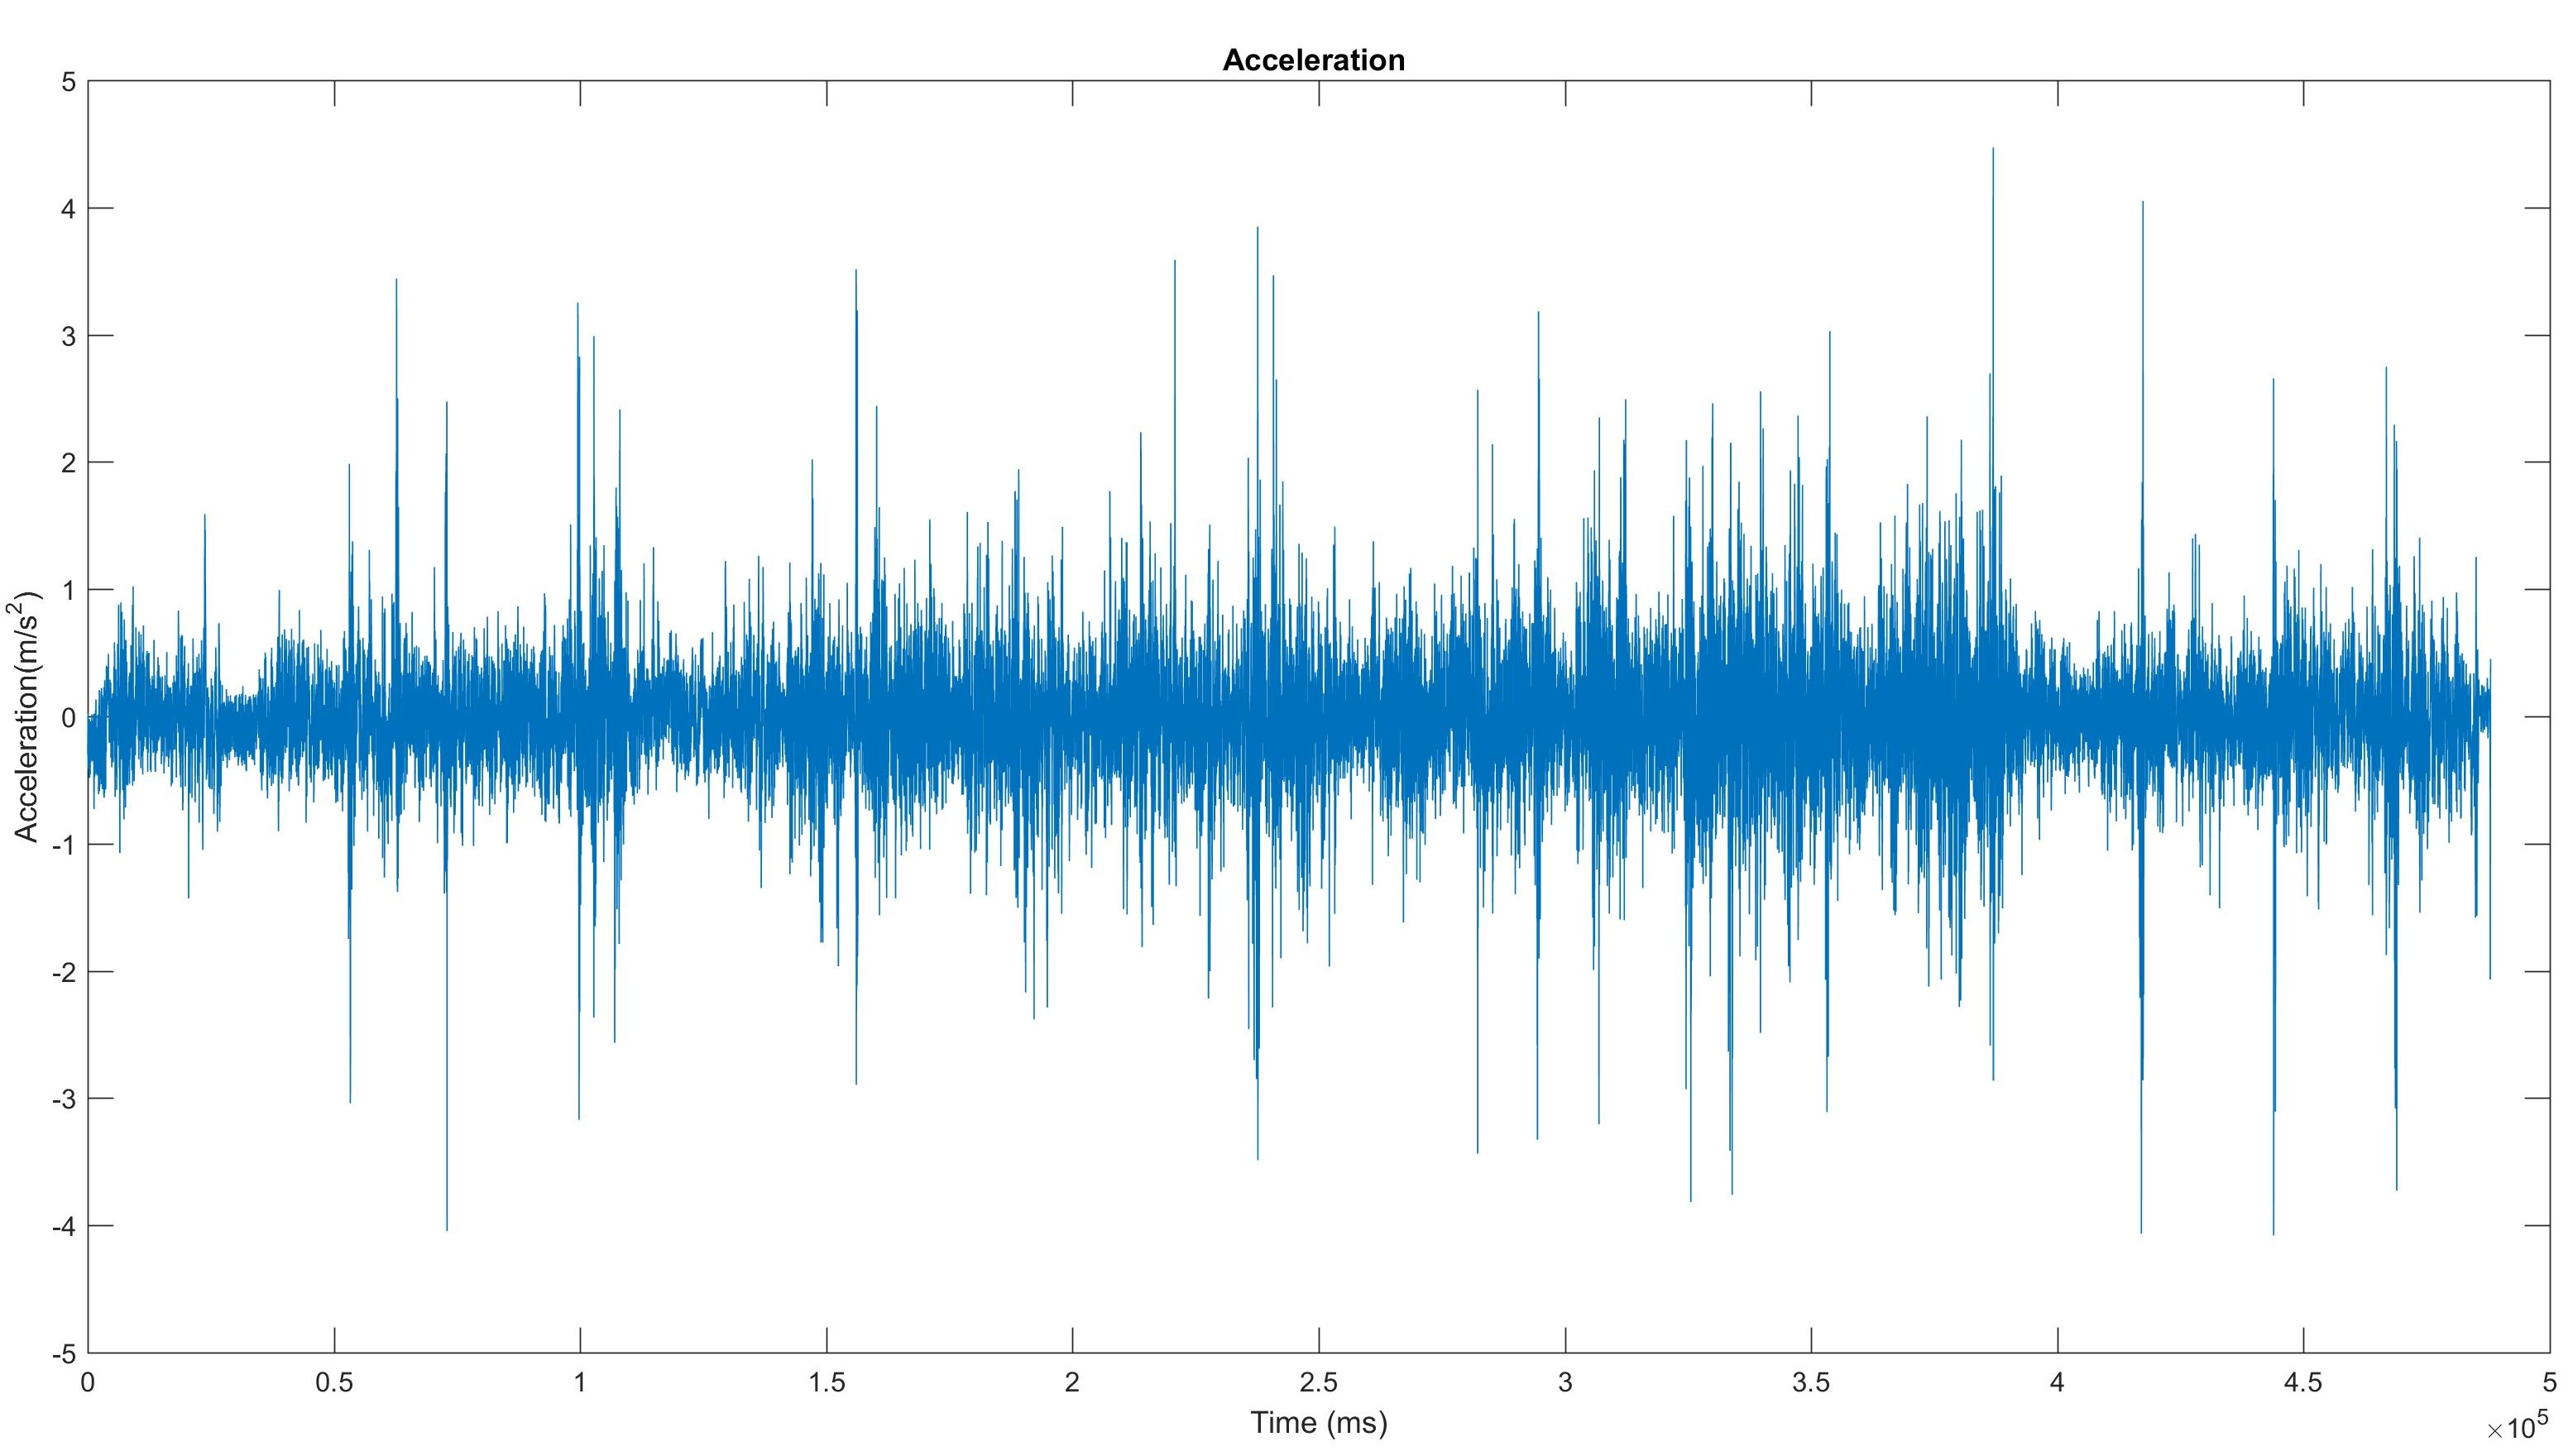
\includegraphics[scale=0.1]{WithRumors}\label{fig:Raw Accelerometer}}    
\subfloat[Without Engine Vibrations]{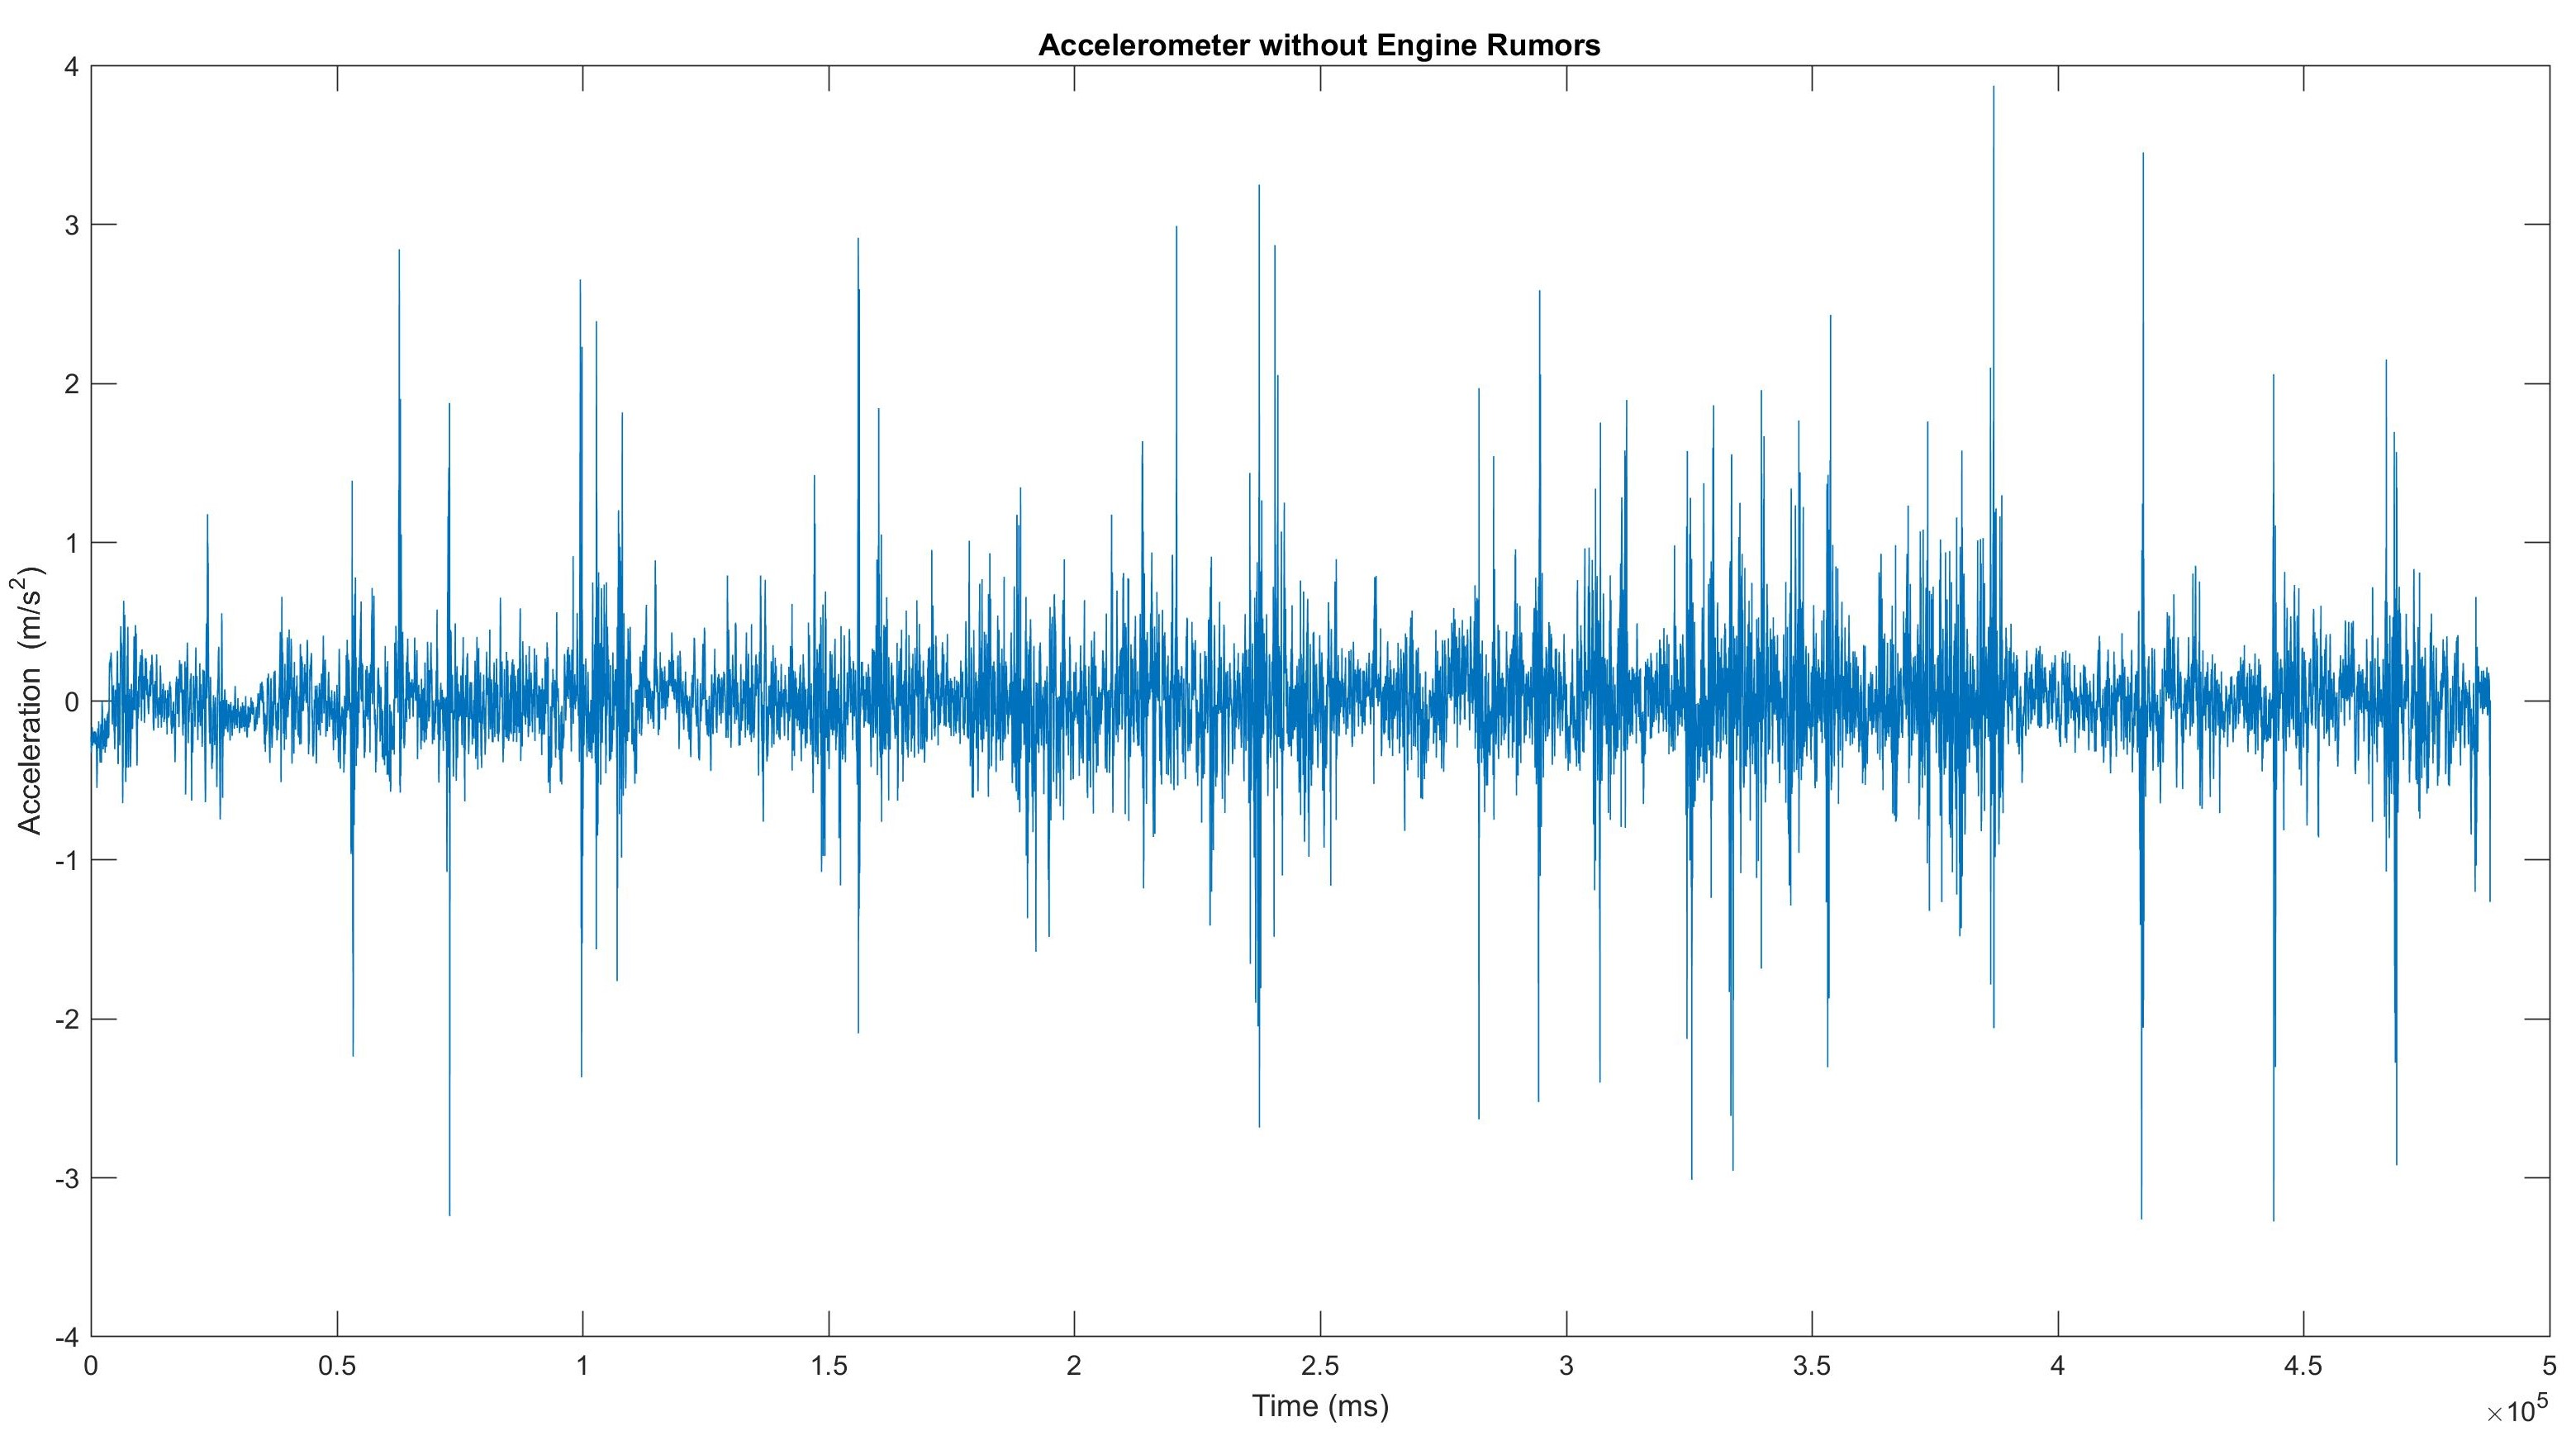
\includegraphics[scale=0.1]{NoRumors}\label{fig:Velocity}}

\centering
\subfloat[Overlapping]{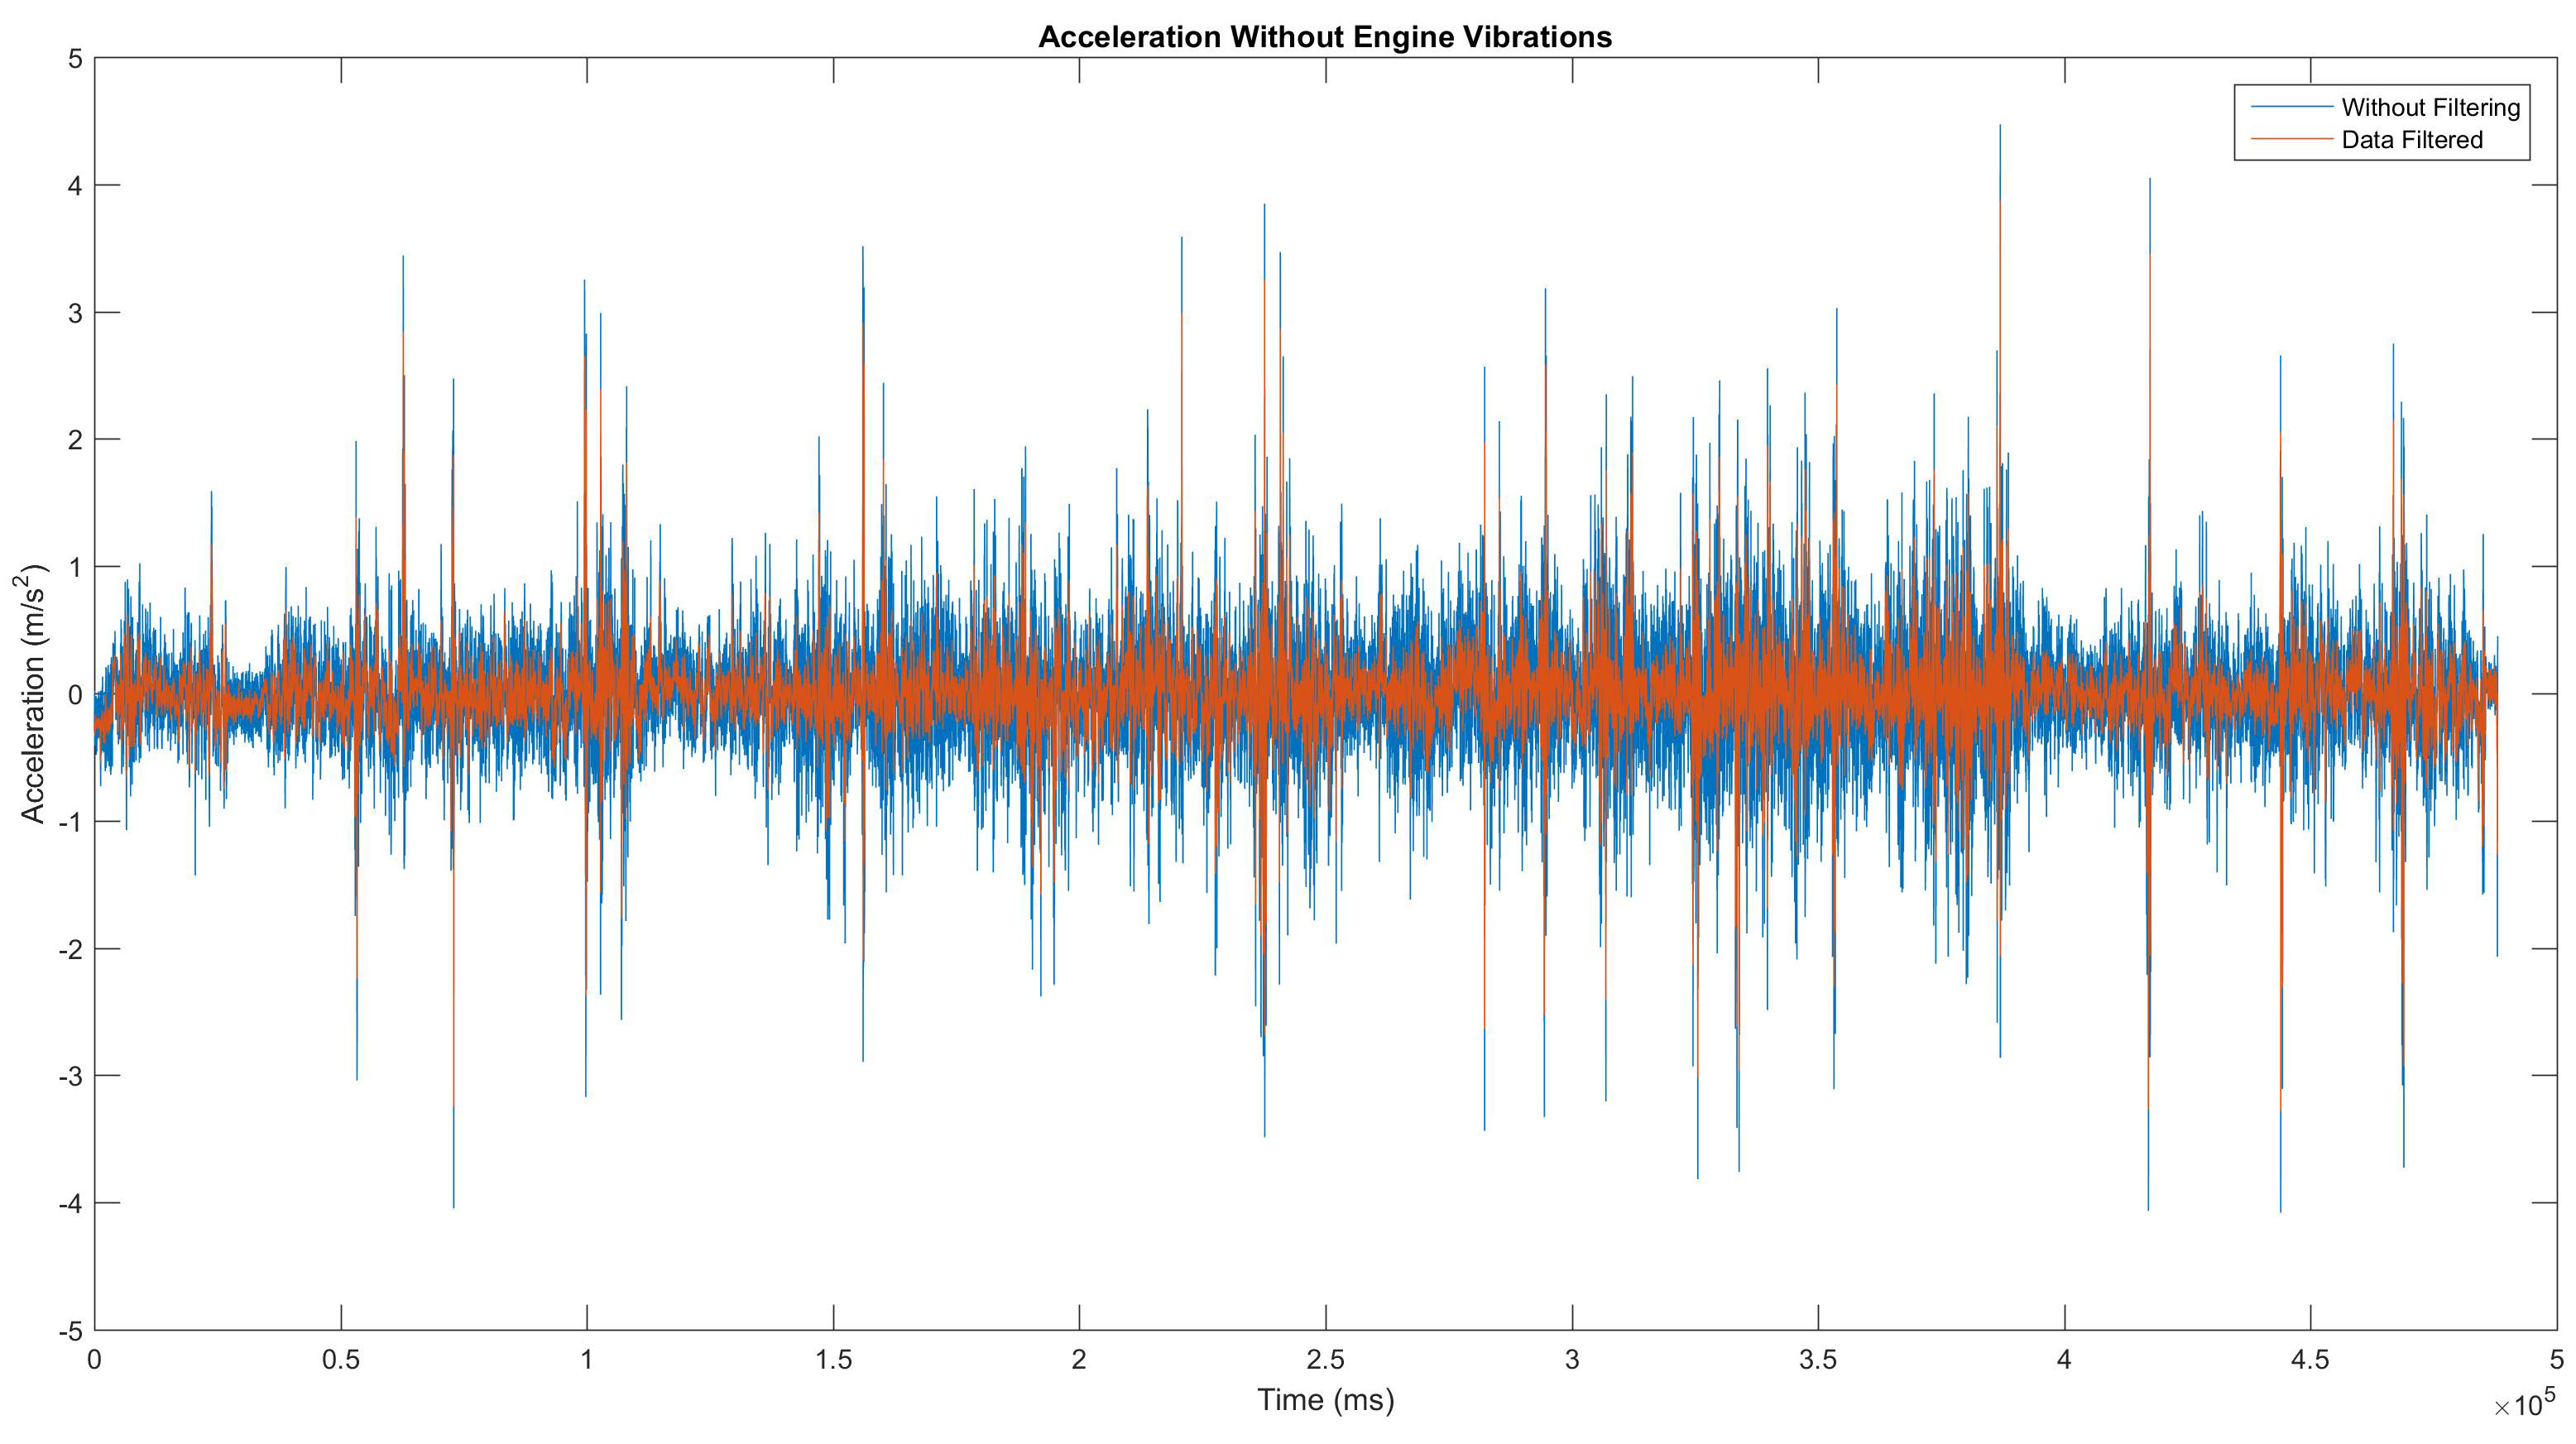
\includegraphics[scale=0.1]{EngineRumors}\label{fig:Sovrapposti}}

The original signal (a) is represent in blue, the filtered signal is represent in orange (b).
 \caption{Application of Engine Vibrations Filter}
  \label{fig:Application of Engine Vibrations Filter.}
\end{figure}

\noindent As is possible to see the signal when filtered it is much lighter, the background noise component produced by the engine is very resonant during the acquisition process, and with this process it is possible to delete it.
\clearpage
\subsubsection{Zero Velocity Filter}
This filter brings attention to the cancellation of certain acceleration values that are associated with zero speed values. Due to several factors, it may happen that while the vehicle is stationary,  because the registration starts even before the vehicle is in motion, or we are in intense traffic situations, stopped at a traffic light, and all other situations that may occur, making us stopped while the smartphone continues to read the data. If any of these conditions occur, the acceleration values can be cancelled, because they would not help us to understand the condition of the road surface.\\\\ \noindent It is possible understand that speed at a given time $(t)$ is equal to $0$ $\si{\km\per\hour}$, thanks to GPS, beacuse during smartphone recordings, gives us the speed of travel.\\\\
\noindent Considering both signals at generic time $(t)$, acceleration ($a_{t}$), and velocity ($v_{t}$), the data series is so modified:
\begin{center}
\[
    \left\{
                \begin{array}{ll}
                  a_{t} = 0; \quad 	if \quad v_{t} = 0 \quad \si{\km\per\hour}\\
                  a_{t} = a_{t}; \quad 	if \quad v_{t} \neq 0 \quad \si{\km\per\hour}\\
                \end{array}
              \right.
\]
\end{center}

\noindent The figure below shows an example of applying this filter to a series of data subject before to Engine Vibrations Filter\ref{Remove Engine Vibrations Filter}.

\begin{figure}[H]	
\subfloat[Acceleration]{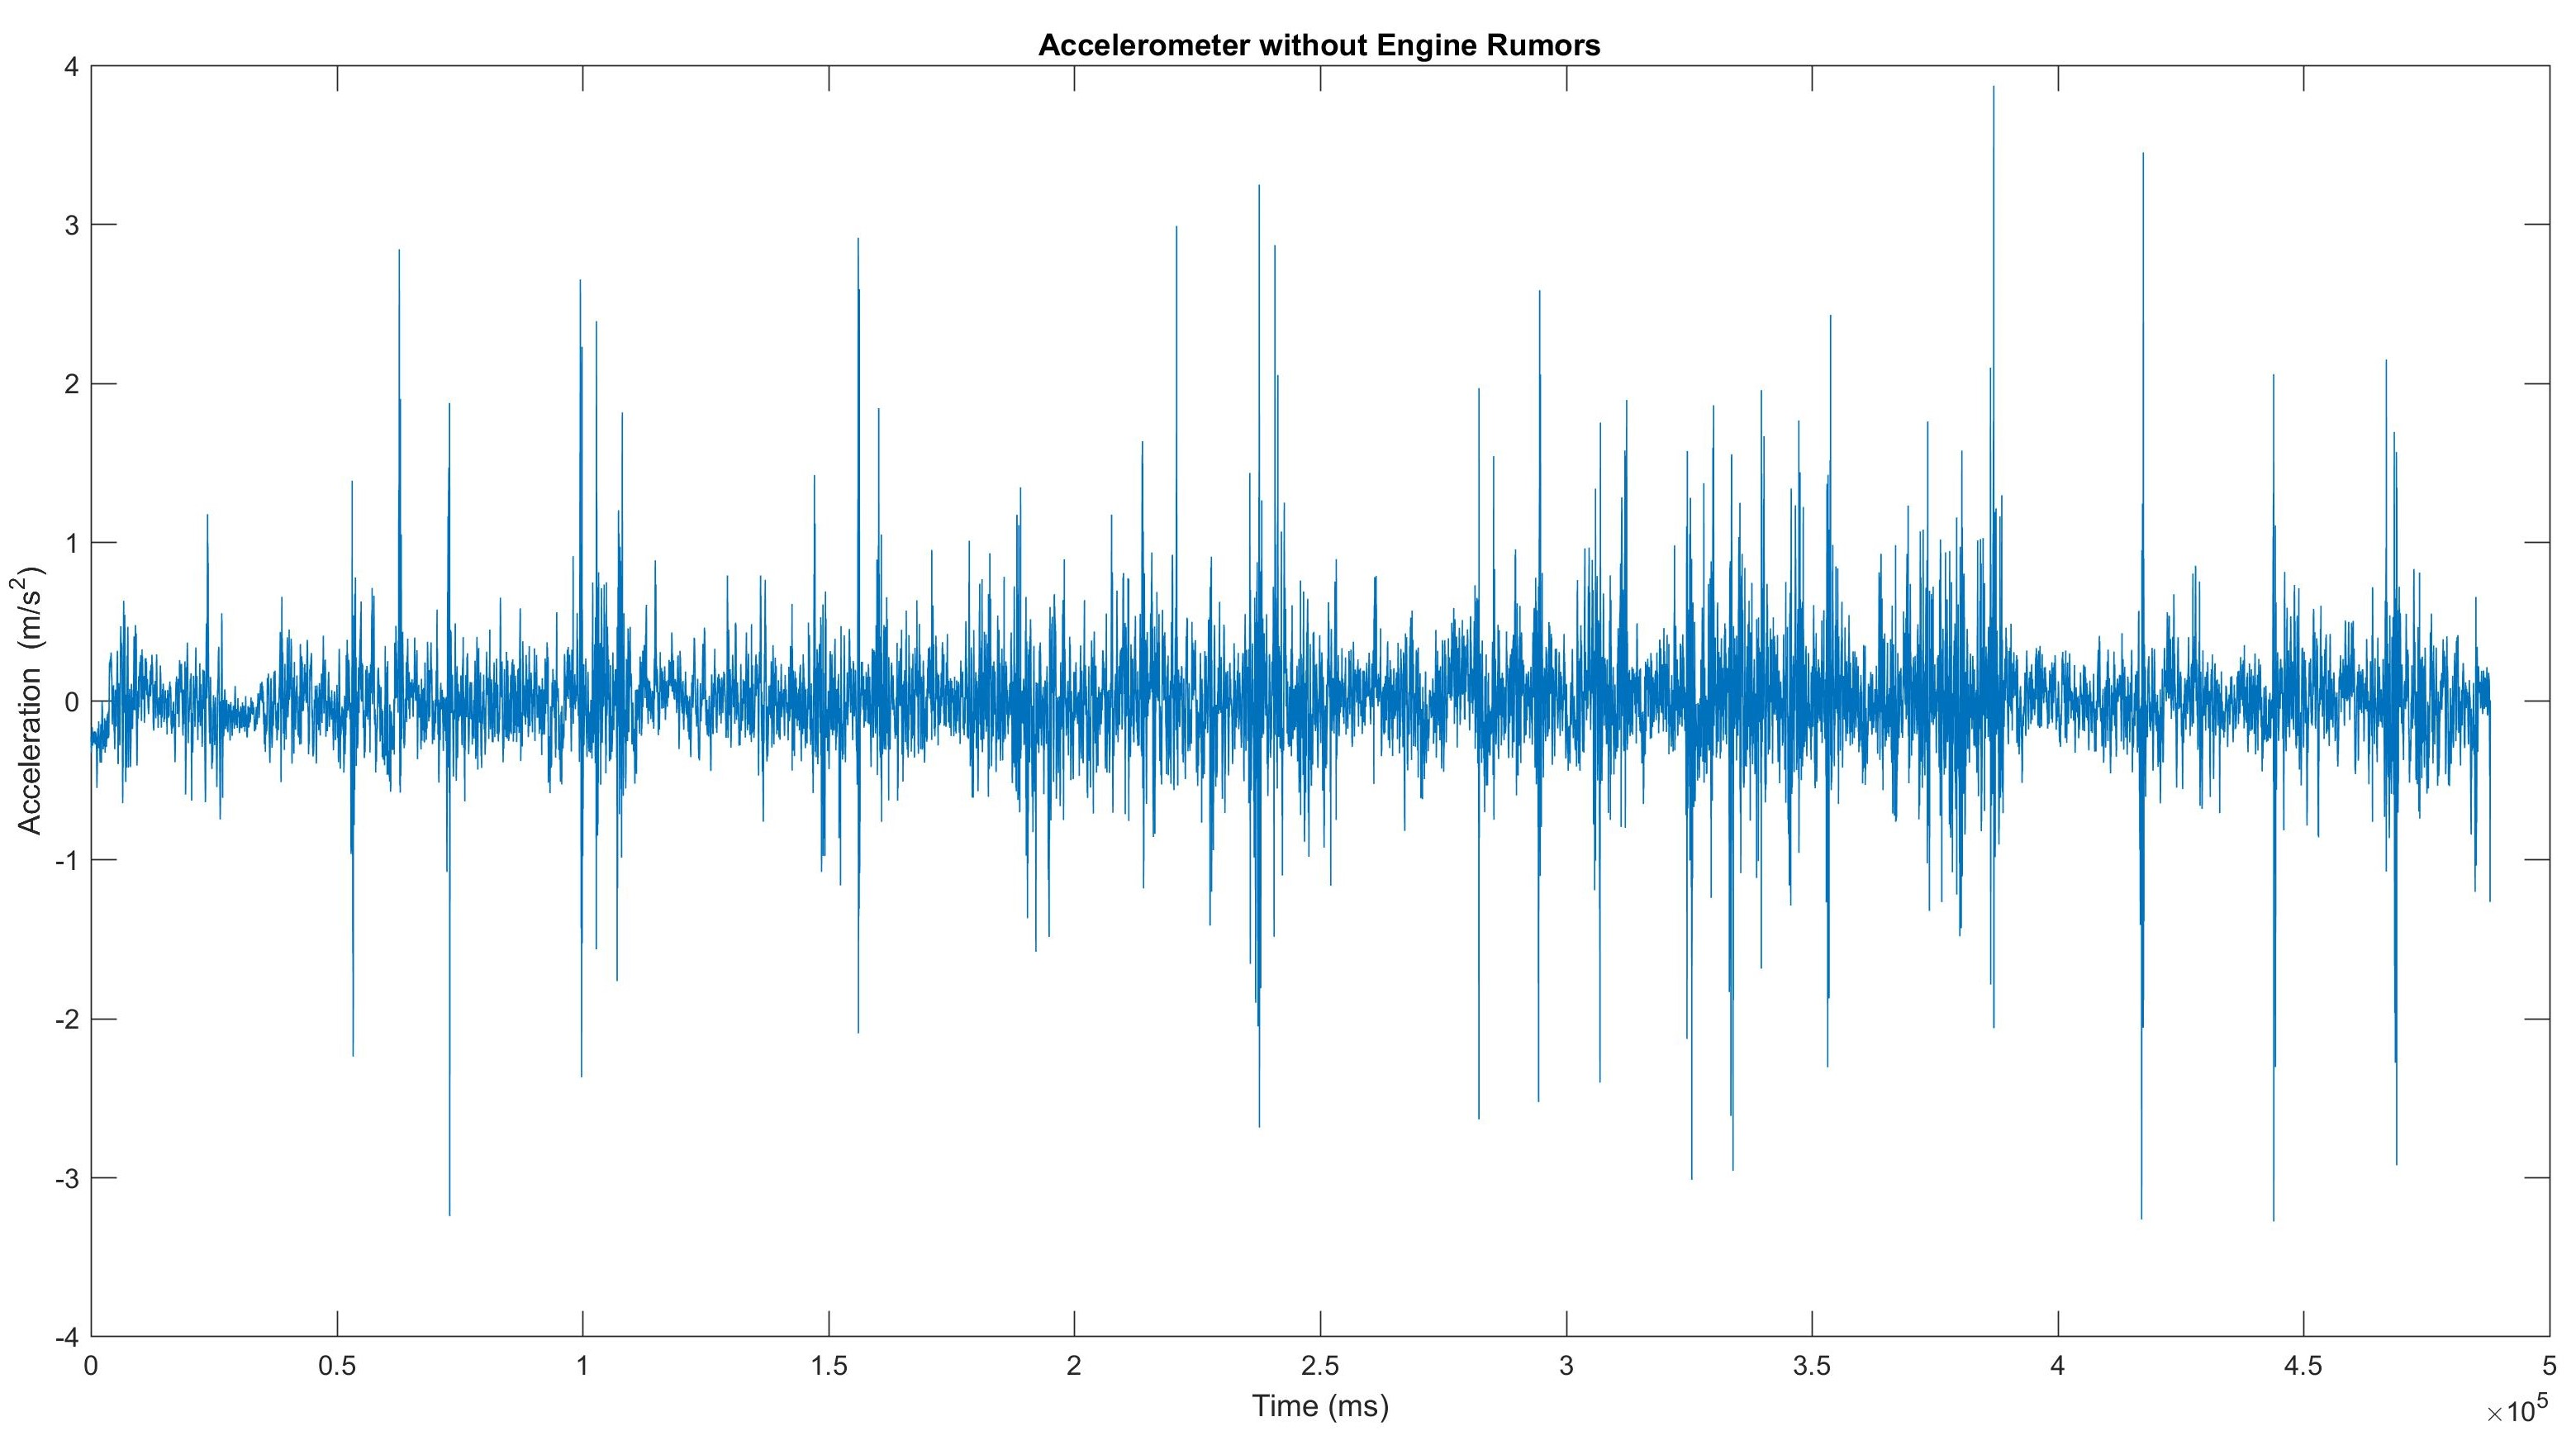
\includegraphics[scale=0.099]{NoRumors}} 
\subfloat[No Zero Velocity]{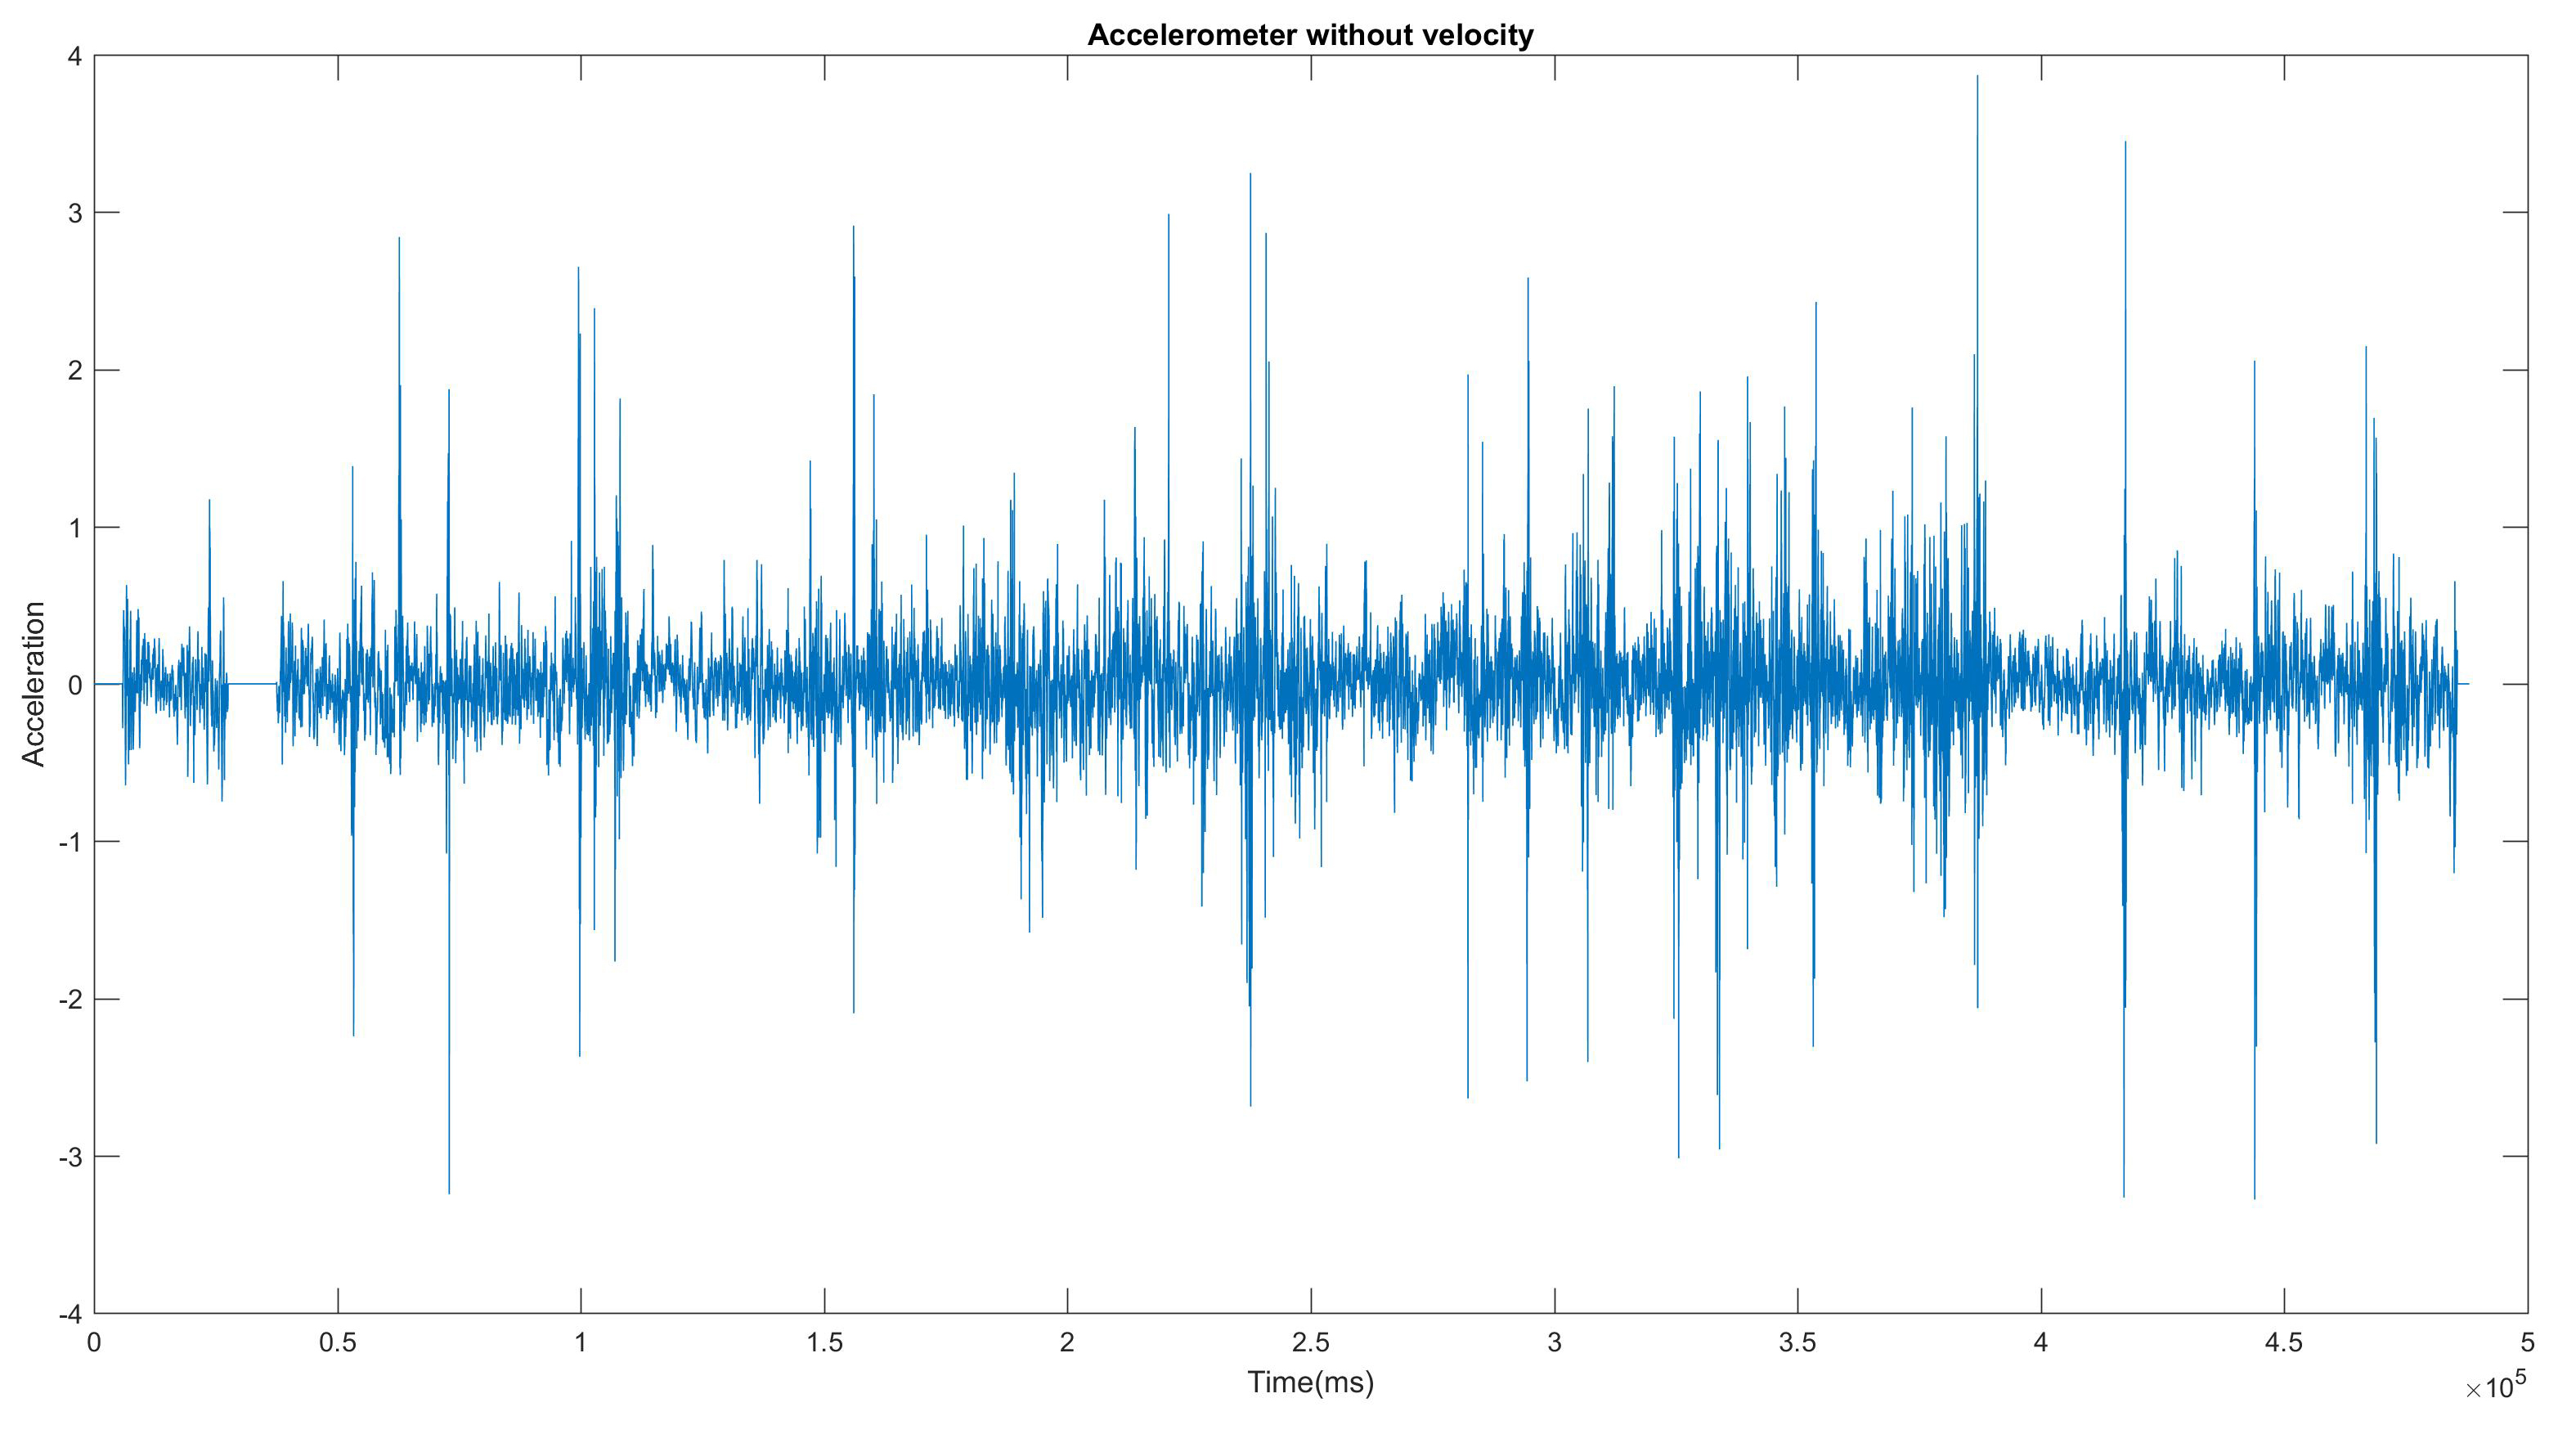
\includegraphics[scale=0.074]{NoVelocity}}

\centering
\subfloat[Overlapping]{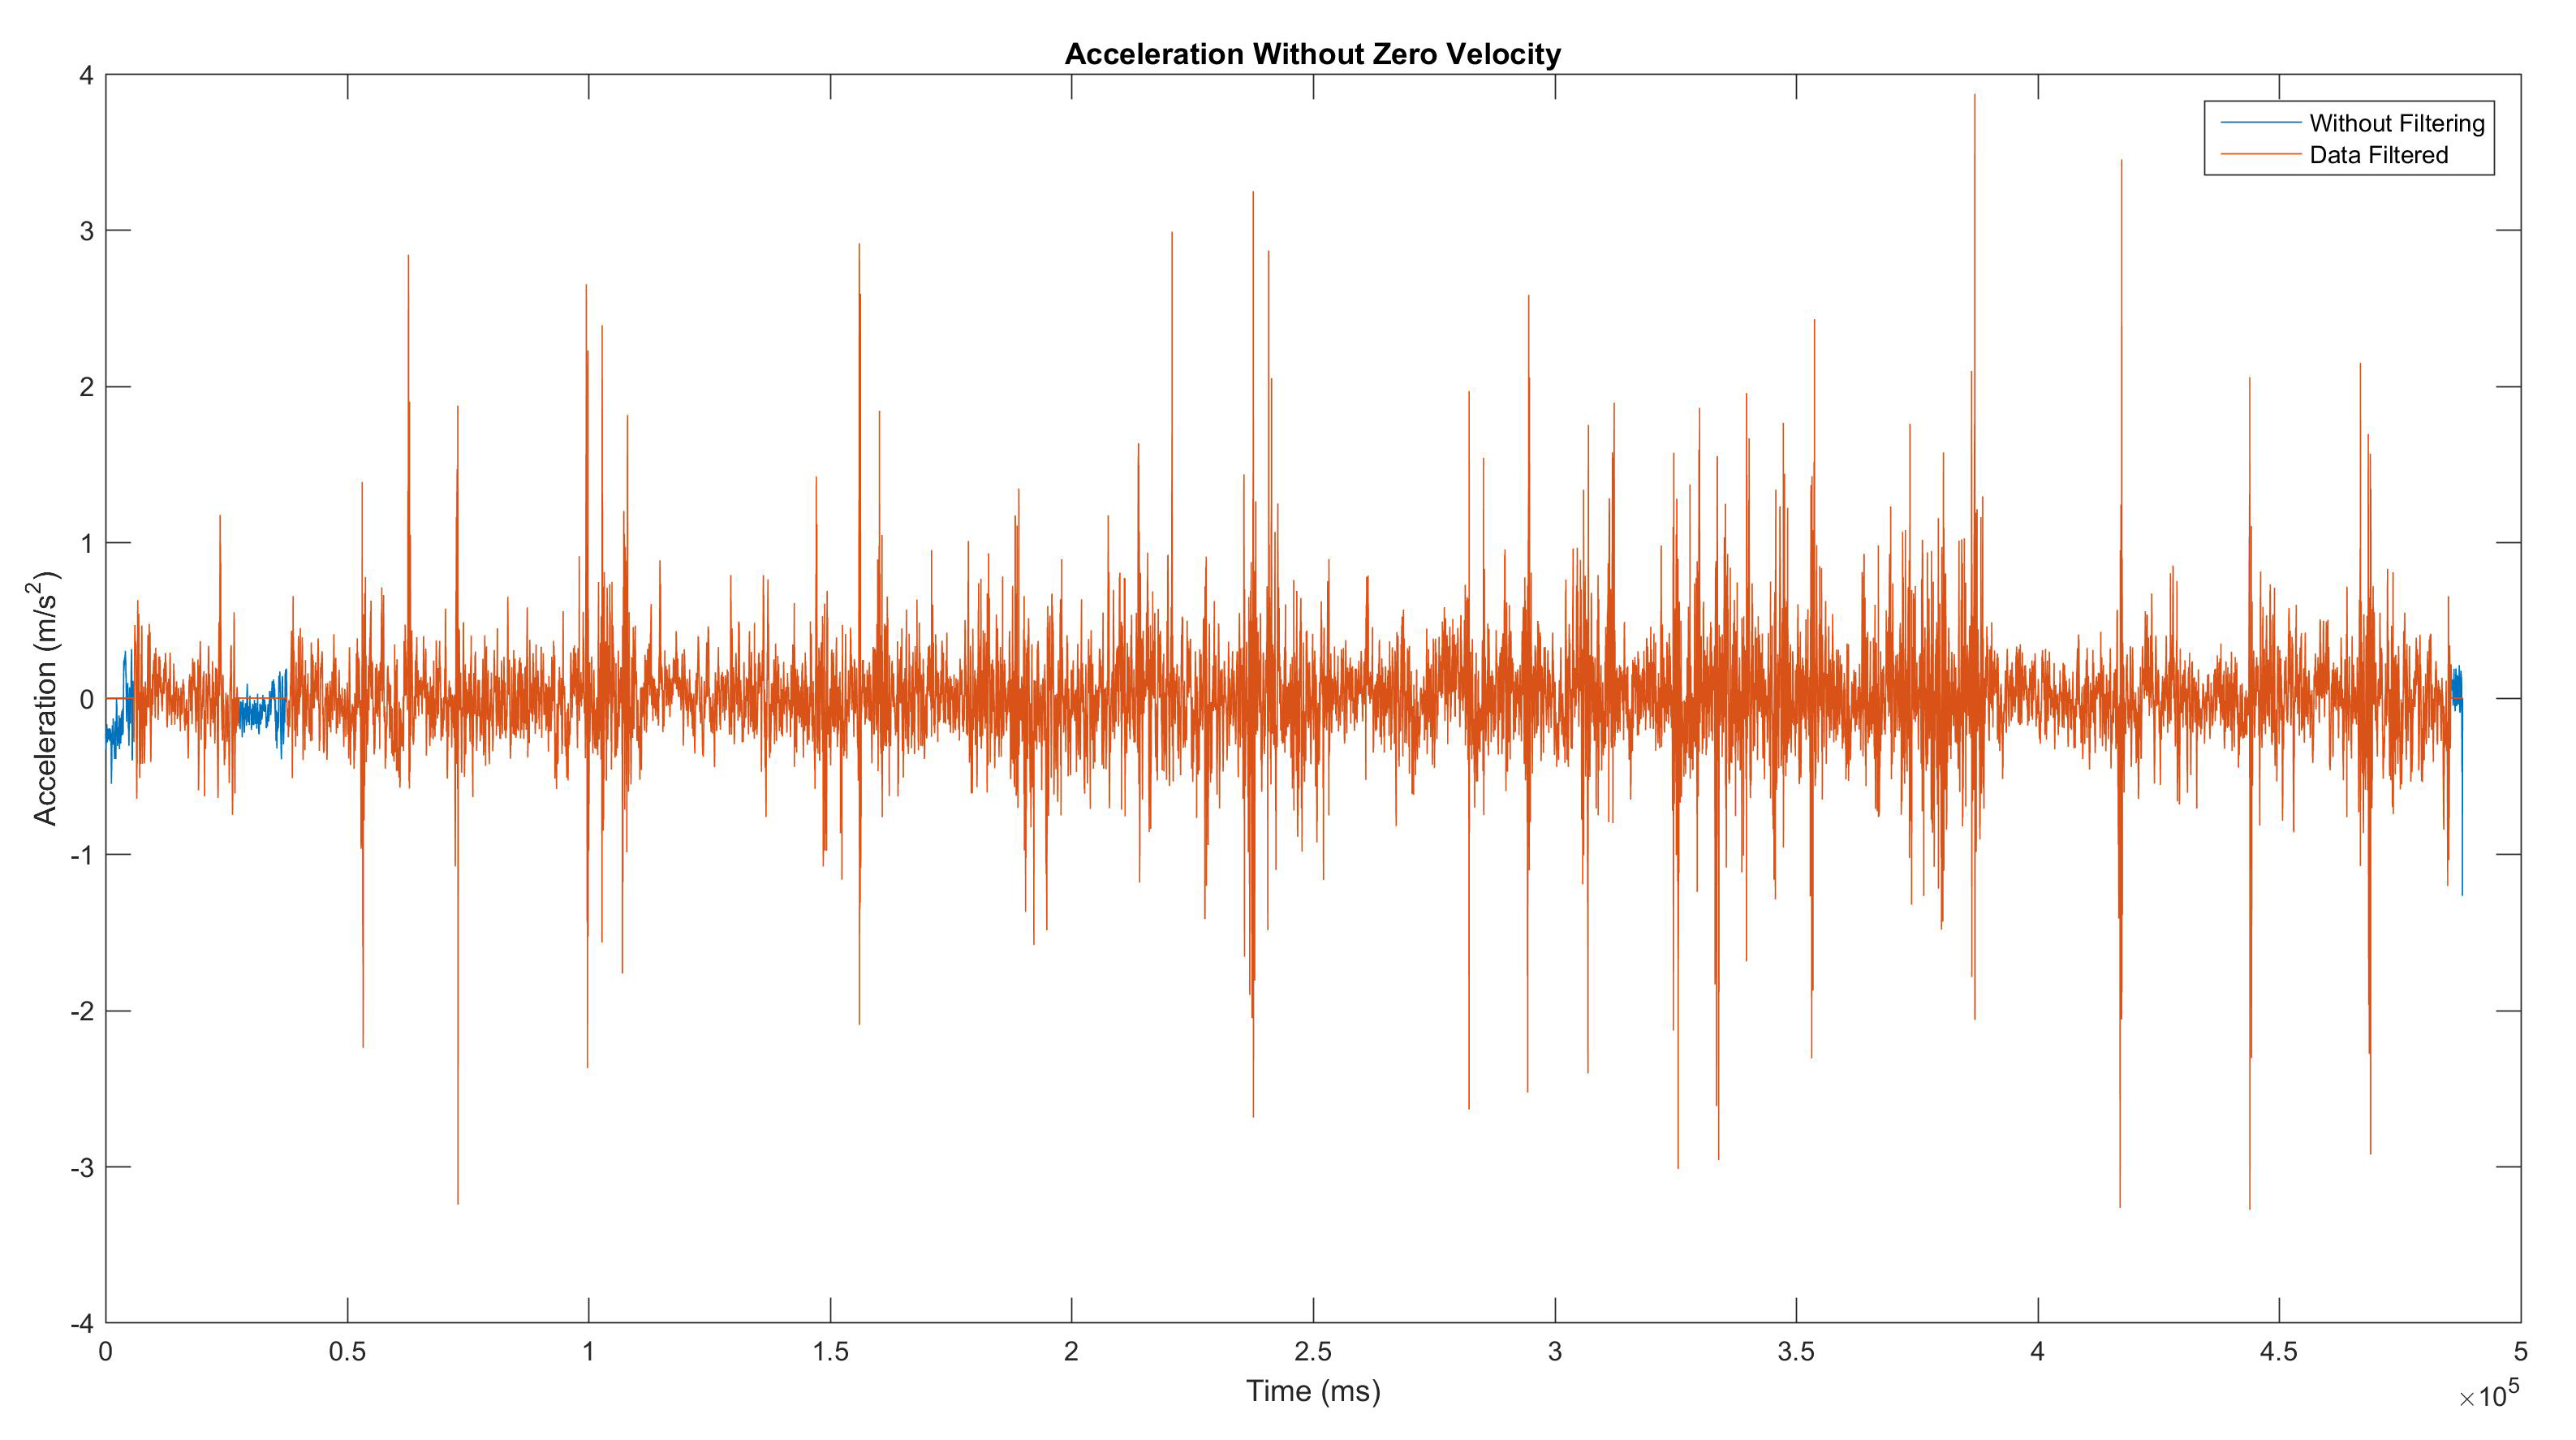
\includegraphics[scale=0.1]{NoVelocitySovrapposte}}

The original signal (a) is represent in blue, the filtered signal is represent in orange (b).

 \caption{Application of Zero Velocity Filter}
  \label{fig:Application of Zero Velocity Filter.}
\end{figure}
\clearpage
\subsection{Digital Filtering} \label{Digital Filtering}
For IRI calculation, vertical displacement is needed, so the accelerometer data must be subject to a double integration process.\\
Unfortunately, accelerometers have an undesired phenomenon named drift associated with them produced by a small DC component\footnote{DC offset is a zero offset compensation. Refers to an electrical signal in which the value is shifted to a certain amount respect to the reference mass.} in the acceleration signal.\\
Ideally, there should be no DC from the accelerometer for the measurement of a vibration. The presence of drift can direct to high integration errors. If the acceleration signal was integrated without any proper filtering, the output could become unlimited over time. The figure \ref{fig:Integration of Raw Data} shows what usually occurs to an acceleration signal after a double integration. Figure \ref{fig:Integration of Raw Data}, is an example of acceleration signal that has a negative DC.\\To resolve the drift problem, a filter can be used to remove the DC component from the acceleration signal. Through filtering before integration, drift errors can be eliminated.\\
For the initial conditions as discusses in \ref{Data Analysis}, a solution is to use filtering.\\  
After the acceleration signal is integrated, it will possibly have a DC component. Again a filter can be used to remove that DC component of the signal. Furthermore, after the velocity signal is integrated to get position, the position signal can be filtered as well.	\\
Filtering is a particular frequency process that attenuates certain bands of frequencies while passing others. These filters will pass the high-frequency content of a signal while rejecting the low. The specifications of a filter are its cutoff frequency, pass-band attenuation, and stop-band attenuation. 
\begin{center}\textit{It is convenient if the filters are identical to each other to simplify the design.}\end{center}


There are two types of filters in the digital area: Infinite Impulse Response (IIR) filters and Finite Impulse Response (FIR) filters. 


\noindent \textit{\textbf{This is applicable as long as the filter does not attenuate frequencies in the signal band. }}

\subsubsection{Finite Impulse Response} \label{Finite Impulse Response}
Finite Impulse Response, (FIR), is a type of digital filter characterised by a finite response, that, it is cancelled at a finite time.\\
A FIR filter is describedd by the following difference equation:

\begin{center}
{\large $y[n] = b_{o} \thinspace x[n] \thinspace  + b_{1} \thinspace  x[n-1] + ... + b_{N} \thinspace  x[n - N] = \thinspace  \sum\limits_{i=0}^{N} \thinspace  b_{i} \thinspace  x[n-i]$}

\end{center}

\noindent Where: 
$x[n]$ is the input signal, $y[n]$ is the output signal, $N$ is the filter order, and $b_{i}$ is the value of the impulse response at instant $i$.\\
This filter is useful for the double integration process. It is recommended to use it because its phase response is linear, which is desired because different frequencies passing through the filter will have the same time delay.\\
A disadvantage is that the order can be very high, and lead to excessive computations.\\
For application to a vehicle road test, there is an interest in processing low frequency signals. So the filter must have a low cutoff frequency with a clear transition band, making the order of the filter high. \\

\clearpage
\paragraph{Moving Average} \leavevmode\\\\
An example of FIR filter is the moving average, commonly used in road pavement profiles, that defines the point $A_{i}$ as the average of the points close to that one, for a base window of length $n$ \cite{little_book}, defined like follow:
\begin{center}
{\large $ A_{i} = \dfrac{1}{n} \thinspace  \sum\limits_{k=i}^{k=i+n} \thinspace  A_{k}$}
\end{center}

\noindent An example of application of the moving average filter is shown in the figure below:
 
\begin{figure}[H]	
\subfloat[Unfiltered]{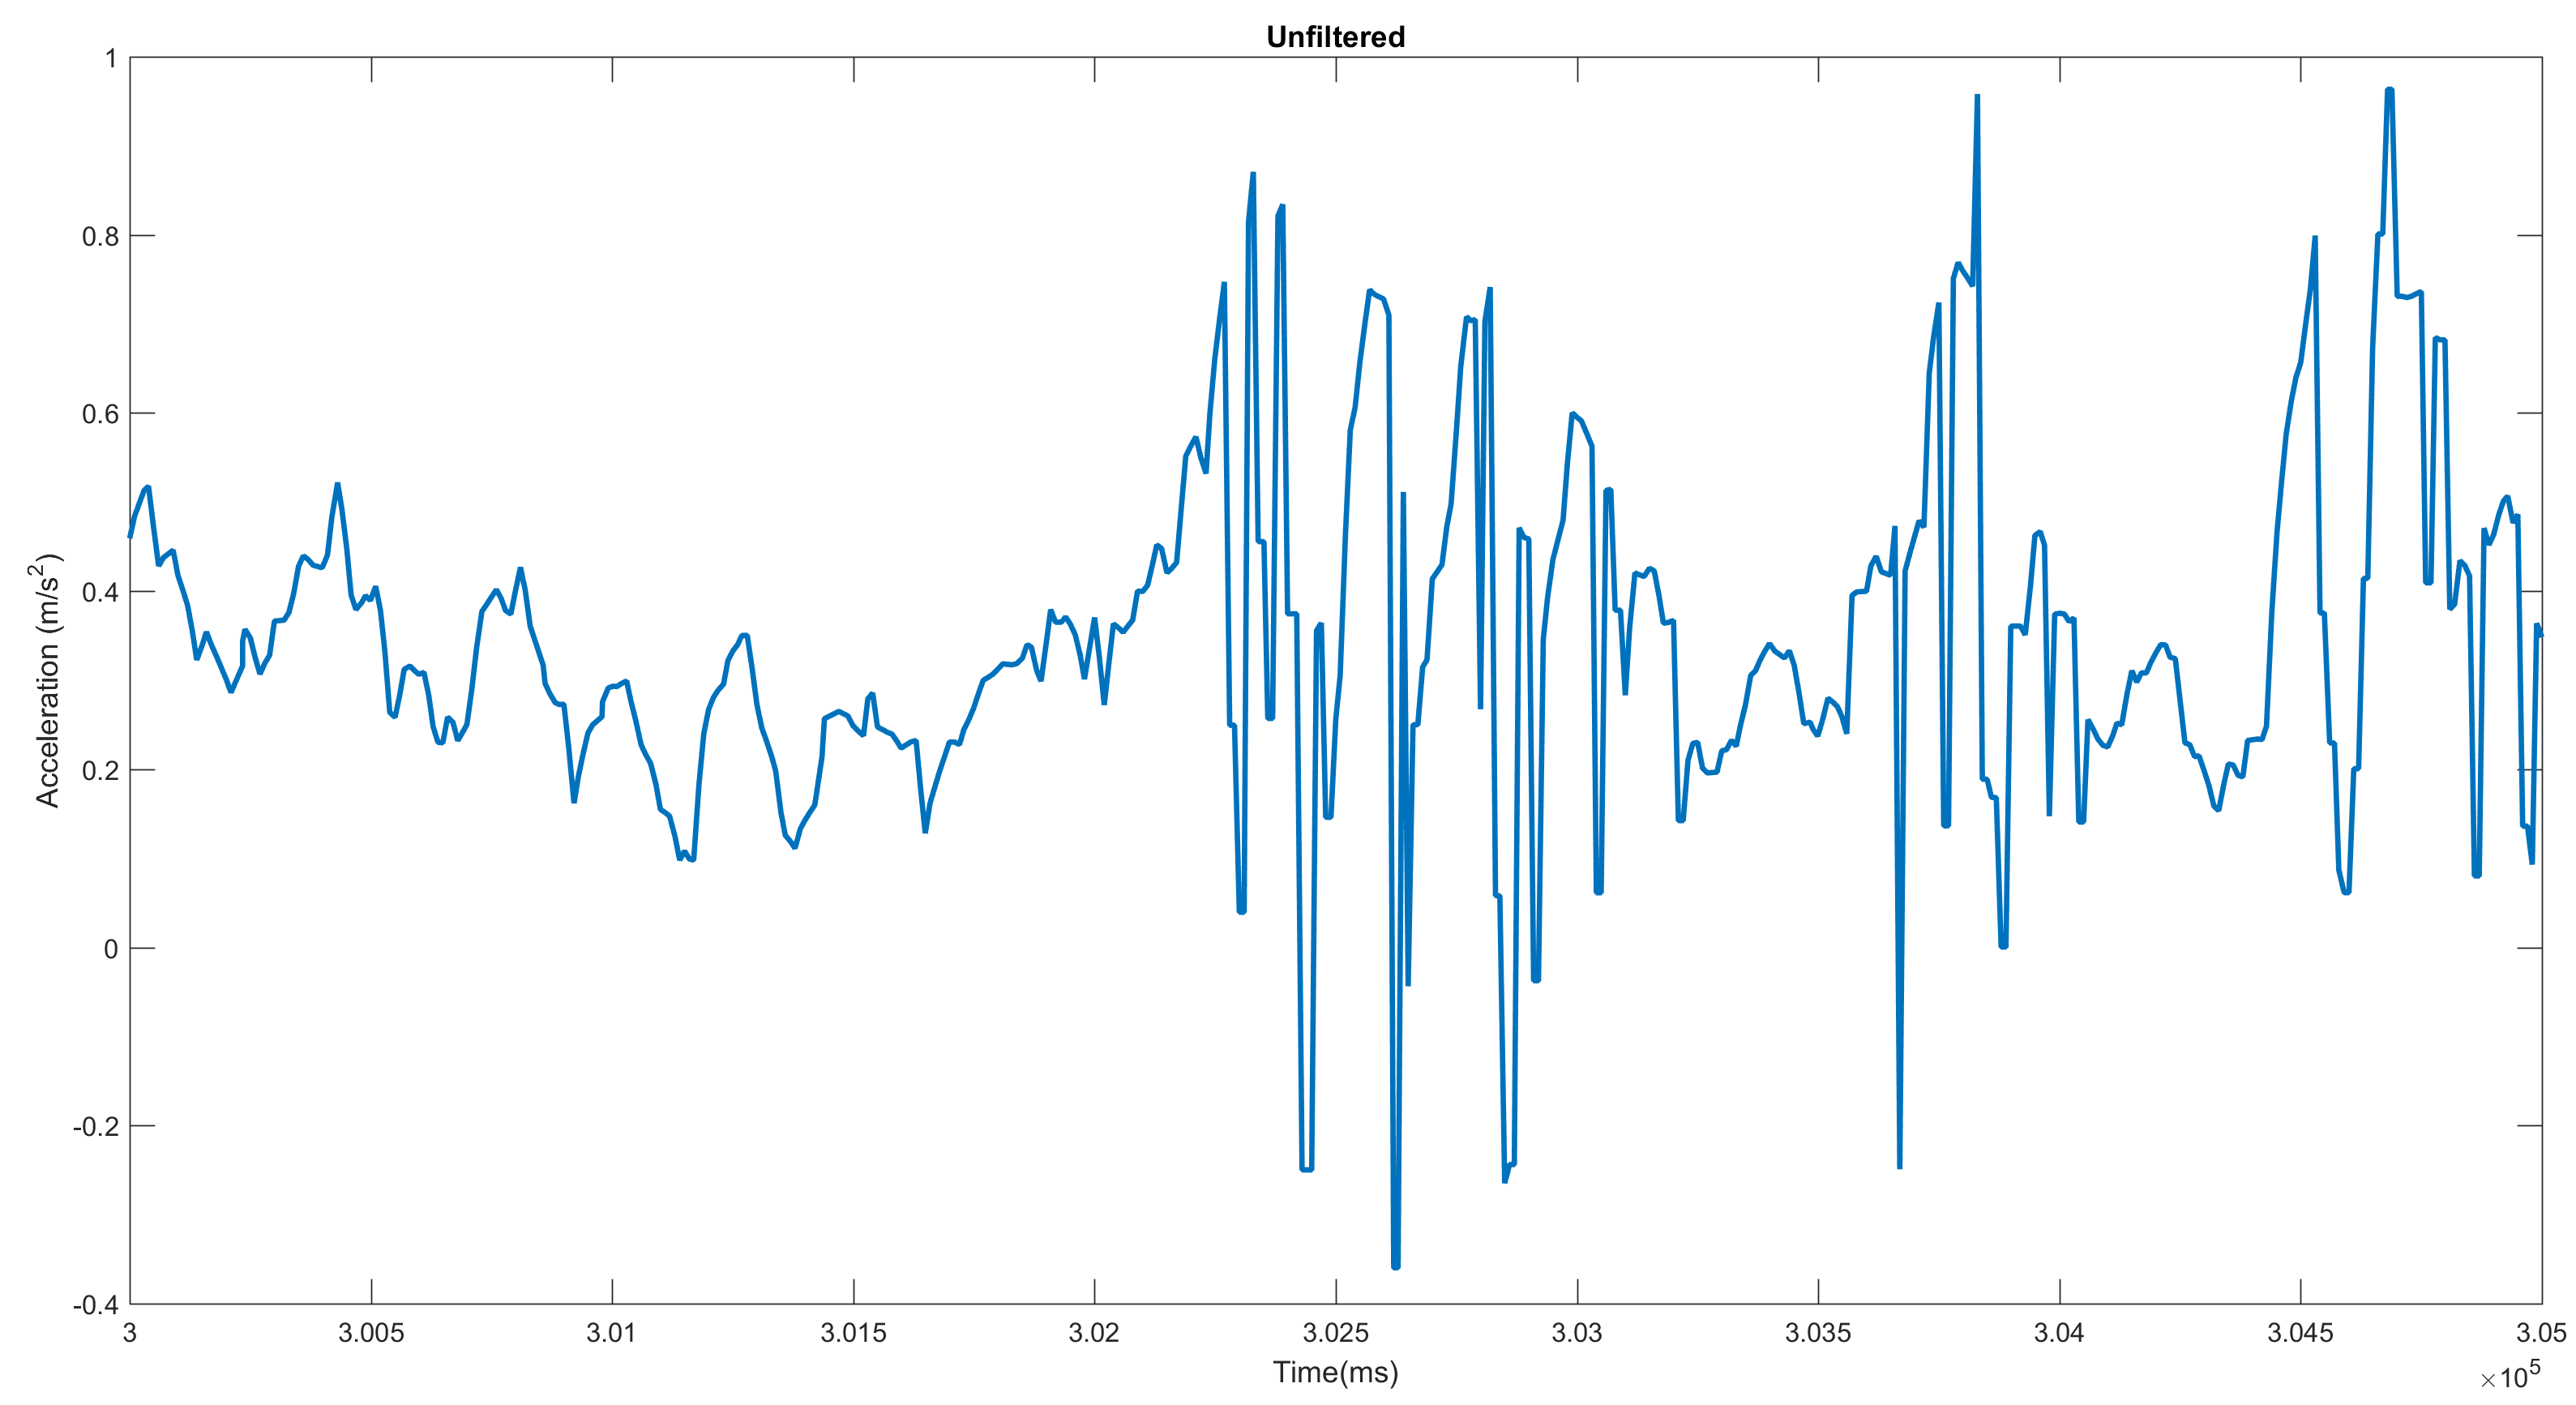
\includegraphics[scale=0.1]{NoMovingFiltered}}    
\subfloat[Filtered]{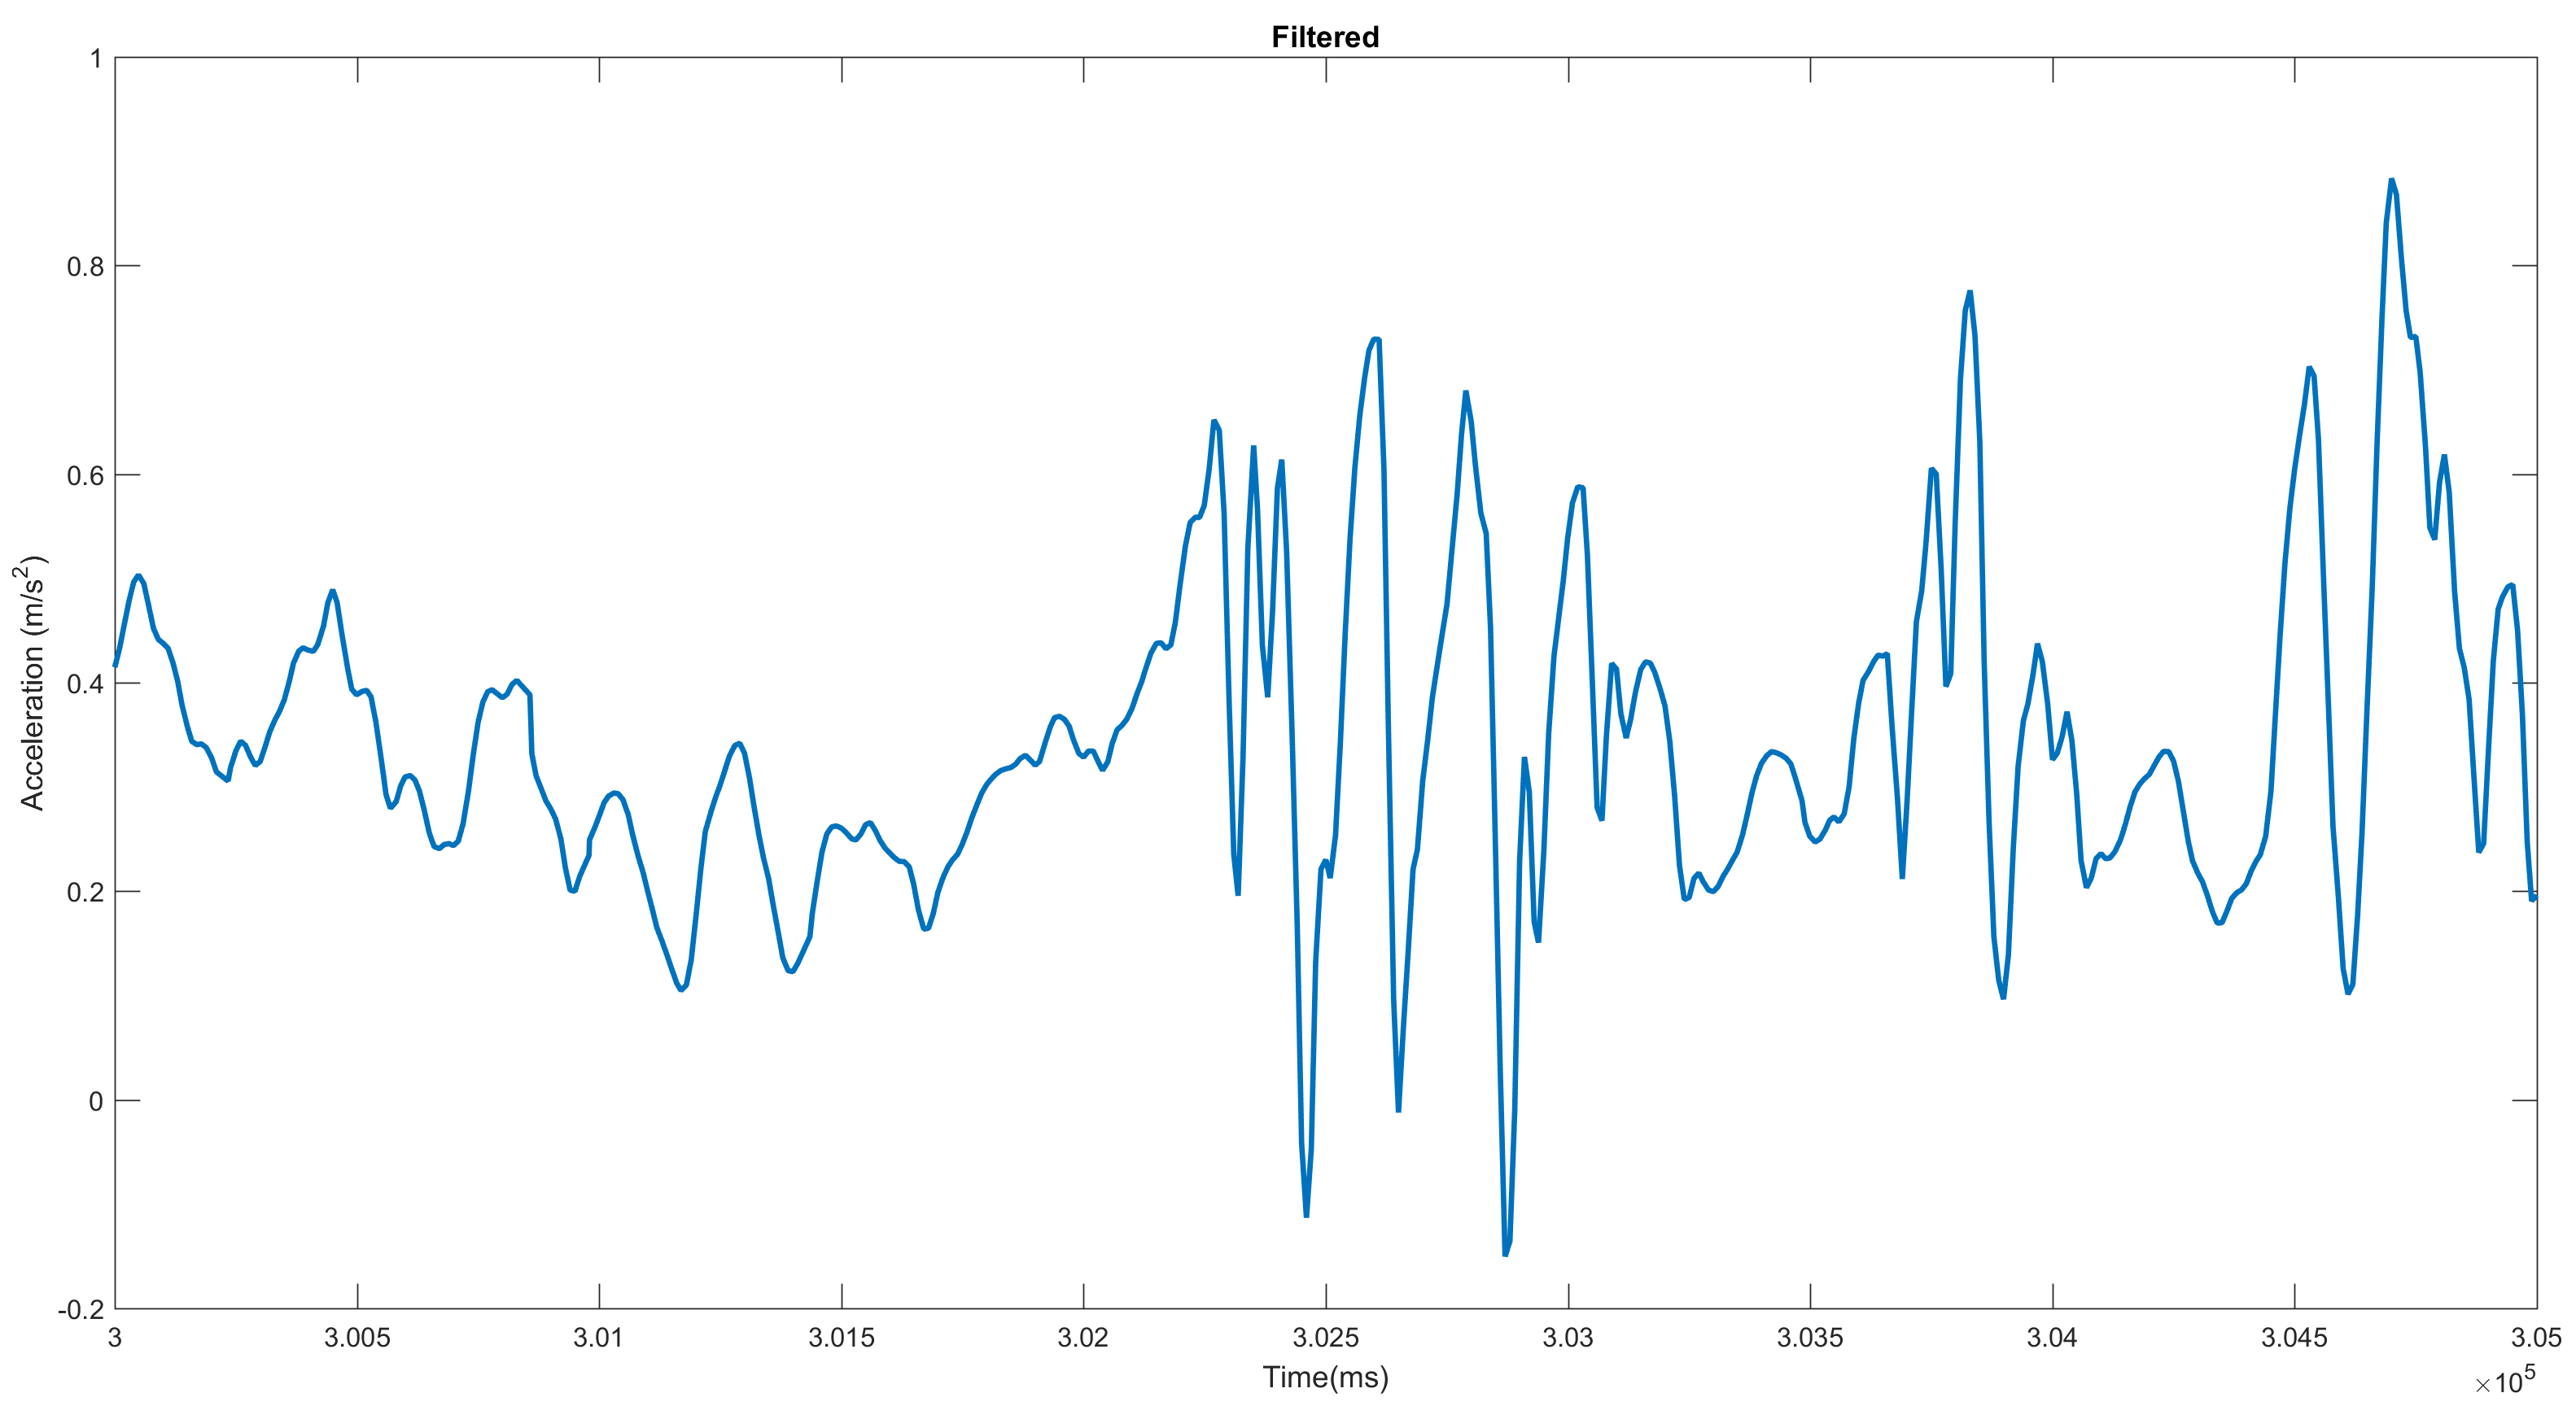
\includegraphics[scale=0.1]{MovingFiltered}}

\centering
\subfloat[Overlapping]{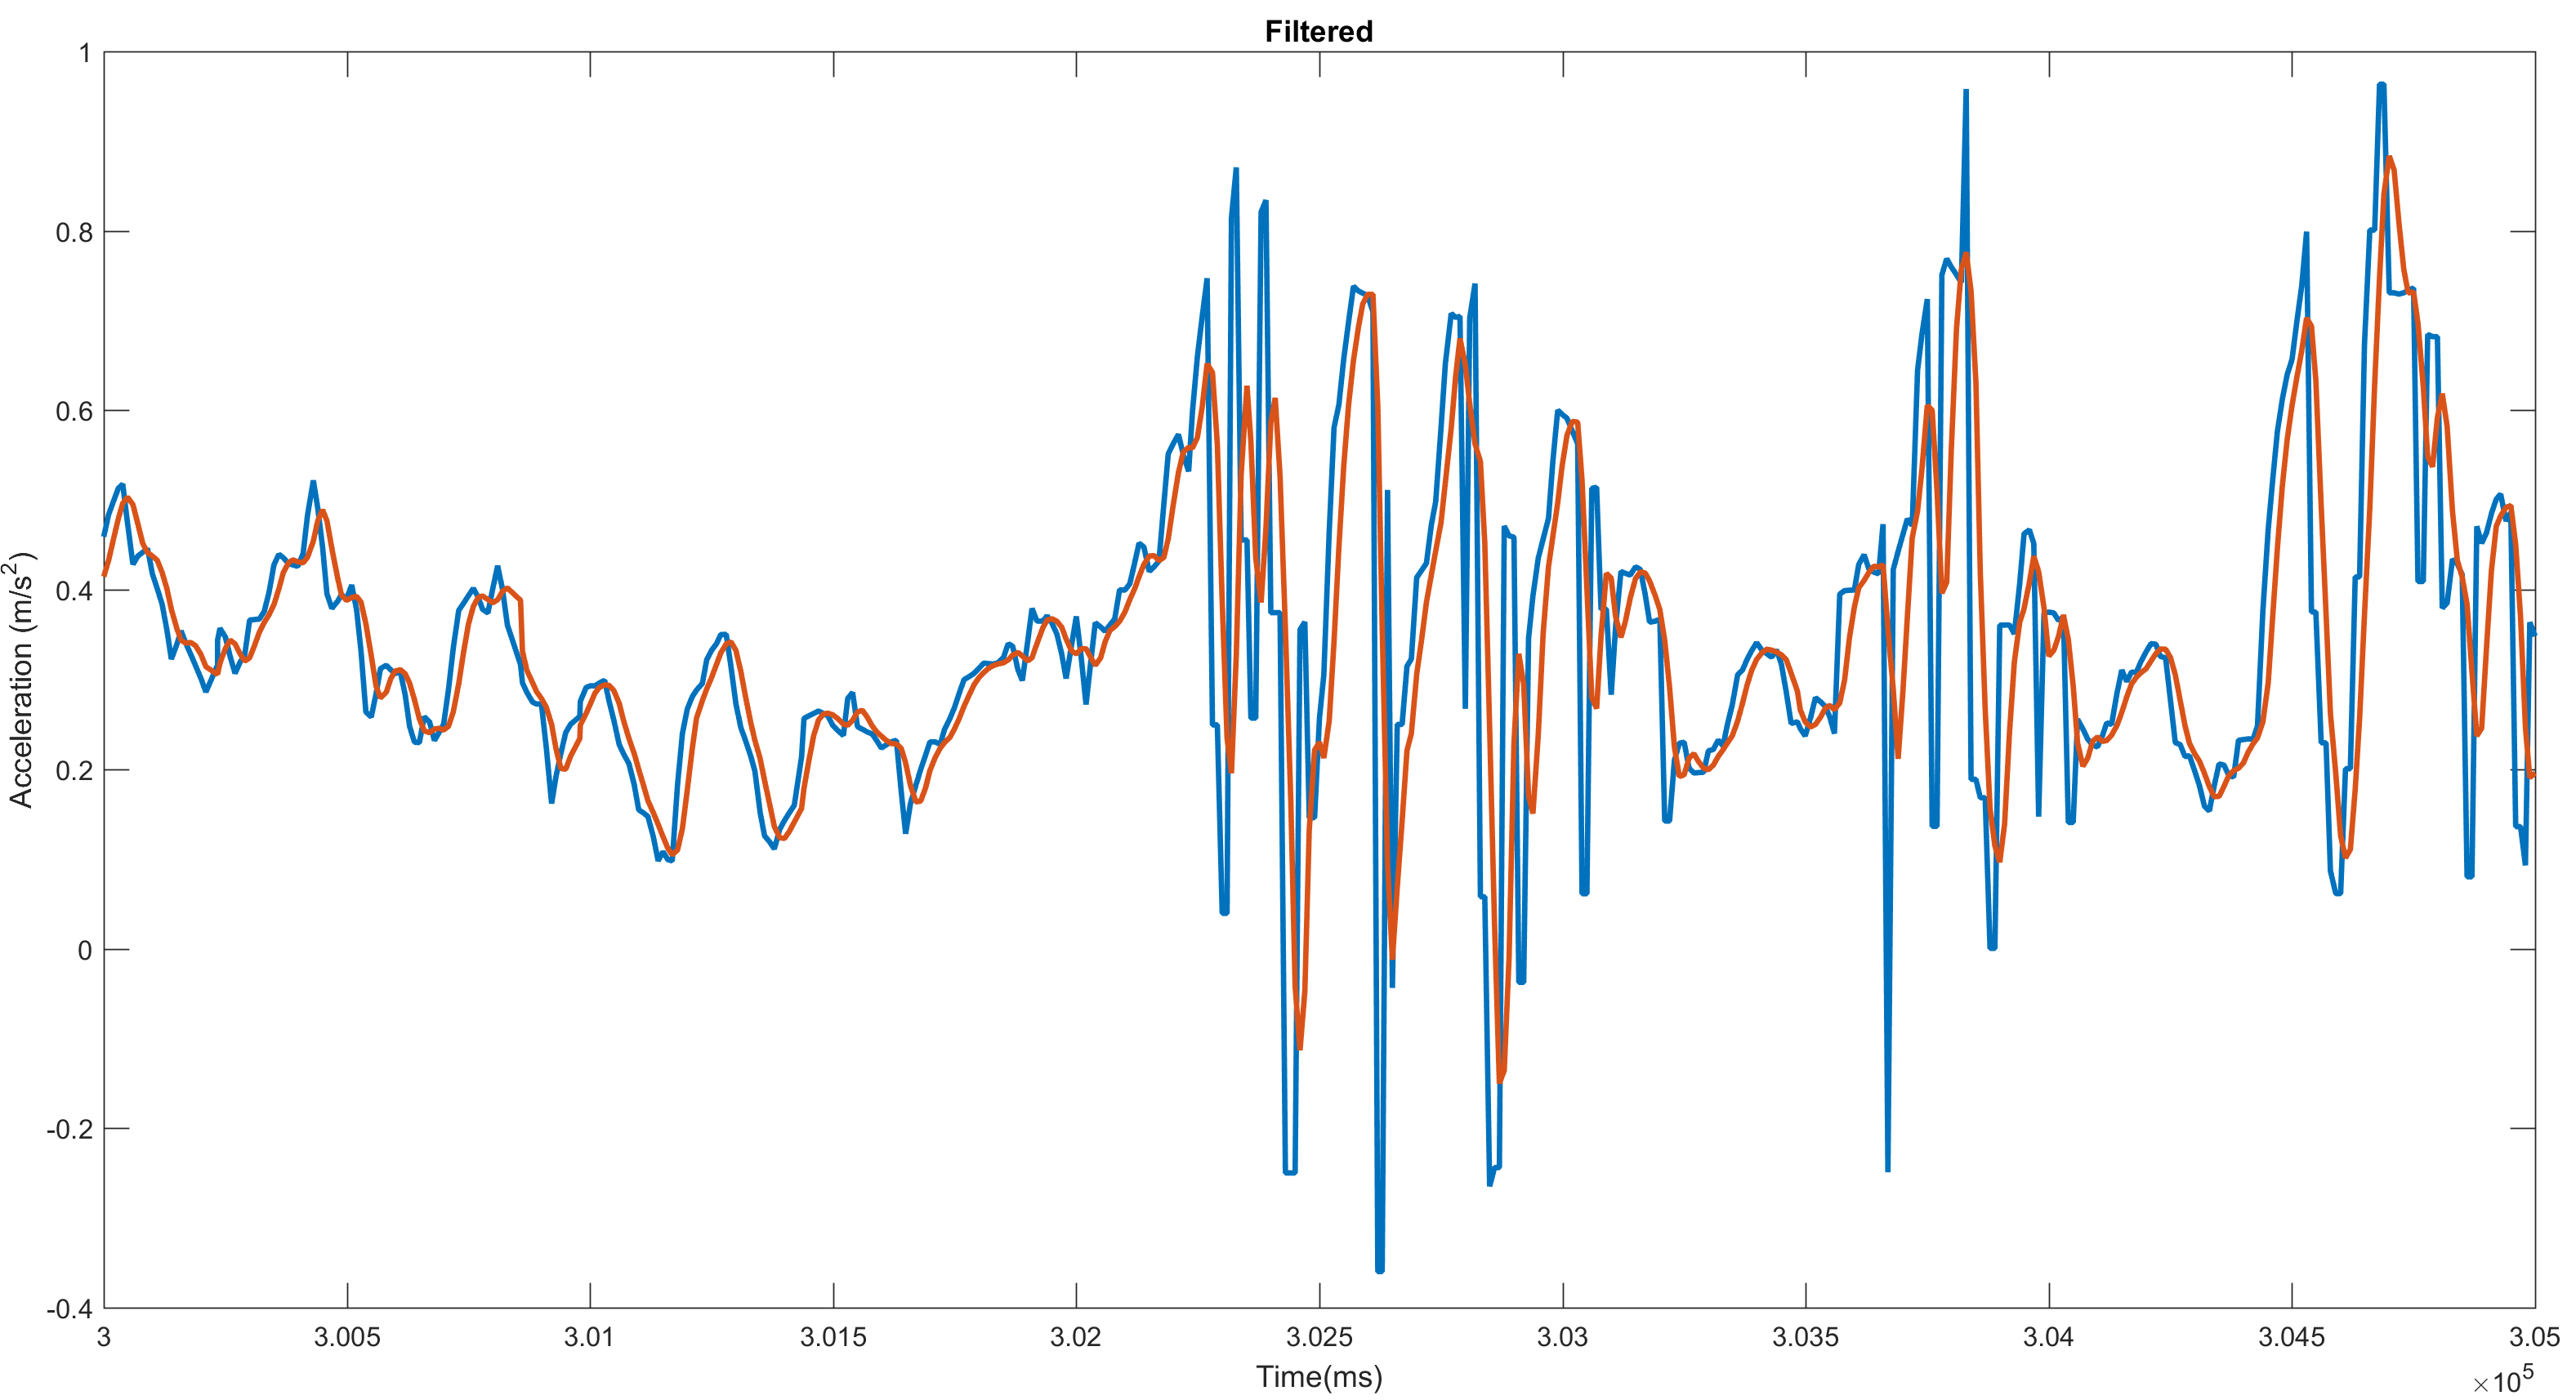
\includegraphics[scale=0.15]{TotalFiltered}}

The original signal (a) is represent in blue, the filtered signal is represent in orange (b).
 \caption{Application of Moving Average Filter}
  \label{fig:Application of Moving Average	 Filter.}
\end{figure}
\subsubsection{Infinite Impulse Response} \label{Infite Impulse Response}
In signals theory, Infinite Impulse Response (IIR) is a dynamic system whose impulsive response is not nothing for an infinite amount of time.\\
IIR filtering, is an alternative approach, that uses a recursive difference equation to represent the filter.

\begin{center}
\begin{large}
$ y[n] = a_{0} \thinspace (\sum\limits_{i=0}^{P}\thinspace  b_{i} \thinspace x[n-1] + \sum\limits_{j=1}^{Q} \thinspace  a_{j} \thinspace  y[n-j])$

\end{large}\end{center}



Where $y[n]$ is the output and $x[n]$ is the input, the output is written as a combination of present and past inputs and past outputs.\\

IIR has an advantage respect FIR filters, regard to the filter order. An IIR filter has a very lower order than FIR, so the computations can be done faster. However, its phase response isn’t linear like the FIR’s response. The physical meaning of this is if a signal is passed through this filter, different frequency components of this signal will be delayed by different lengths of time, causing distortion. \\
There is a way to overcome the problem of having a non-linear phase with the IIR filter. 
Filter the signal, time reverses the signal, and filter it again with the same filter. A MATLAB command (filtfilt)  does this operation automatically. 


\section{GPS points division} \label{GPS points division}
Another problem to fix is the way geolocation points are identified.\\
As discussed in Chapter 3, (GPS section, page), GPS records the data at a frequency of $1$ $Hz$ (every second), however, the acceleration data as we have seen in our case are recorded at $100$ $Hz$ (every $10$ $ms$).\\
For every GPS recording, $100$ acceleration data will be registered. This puts us in front of a problem because if we want to map the road surface correctly, GPS data need to be very close to each other.\\
To understand better this factor, two different GPS coordinates were identified:

\begin{center}
 $Start = (Latitude_{start}, Longitude_{start})$\\
 $End = (Longitude_{end}, Longitude_{end})$
\end{center}

\noindent Show on the figure below:
\vspace{0.15cm}
\begin{figure}[H]	

\centering
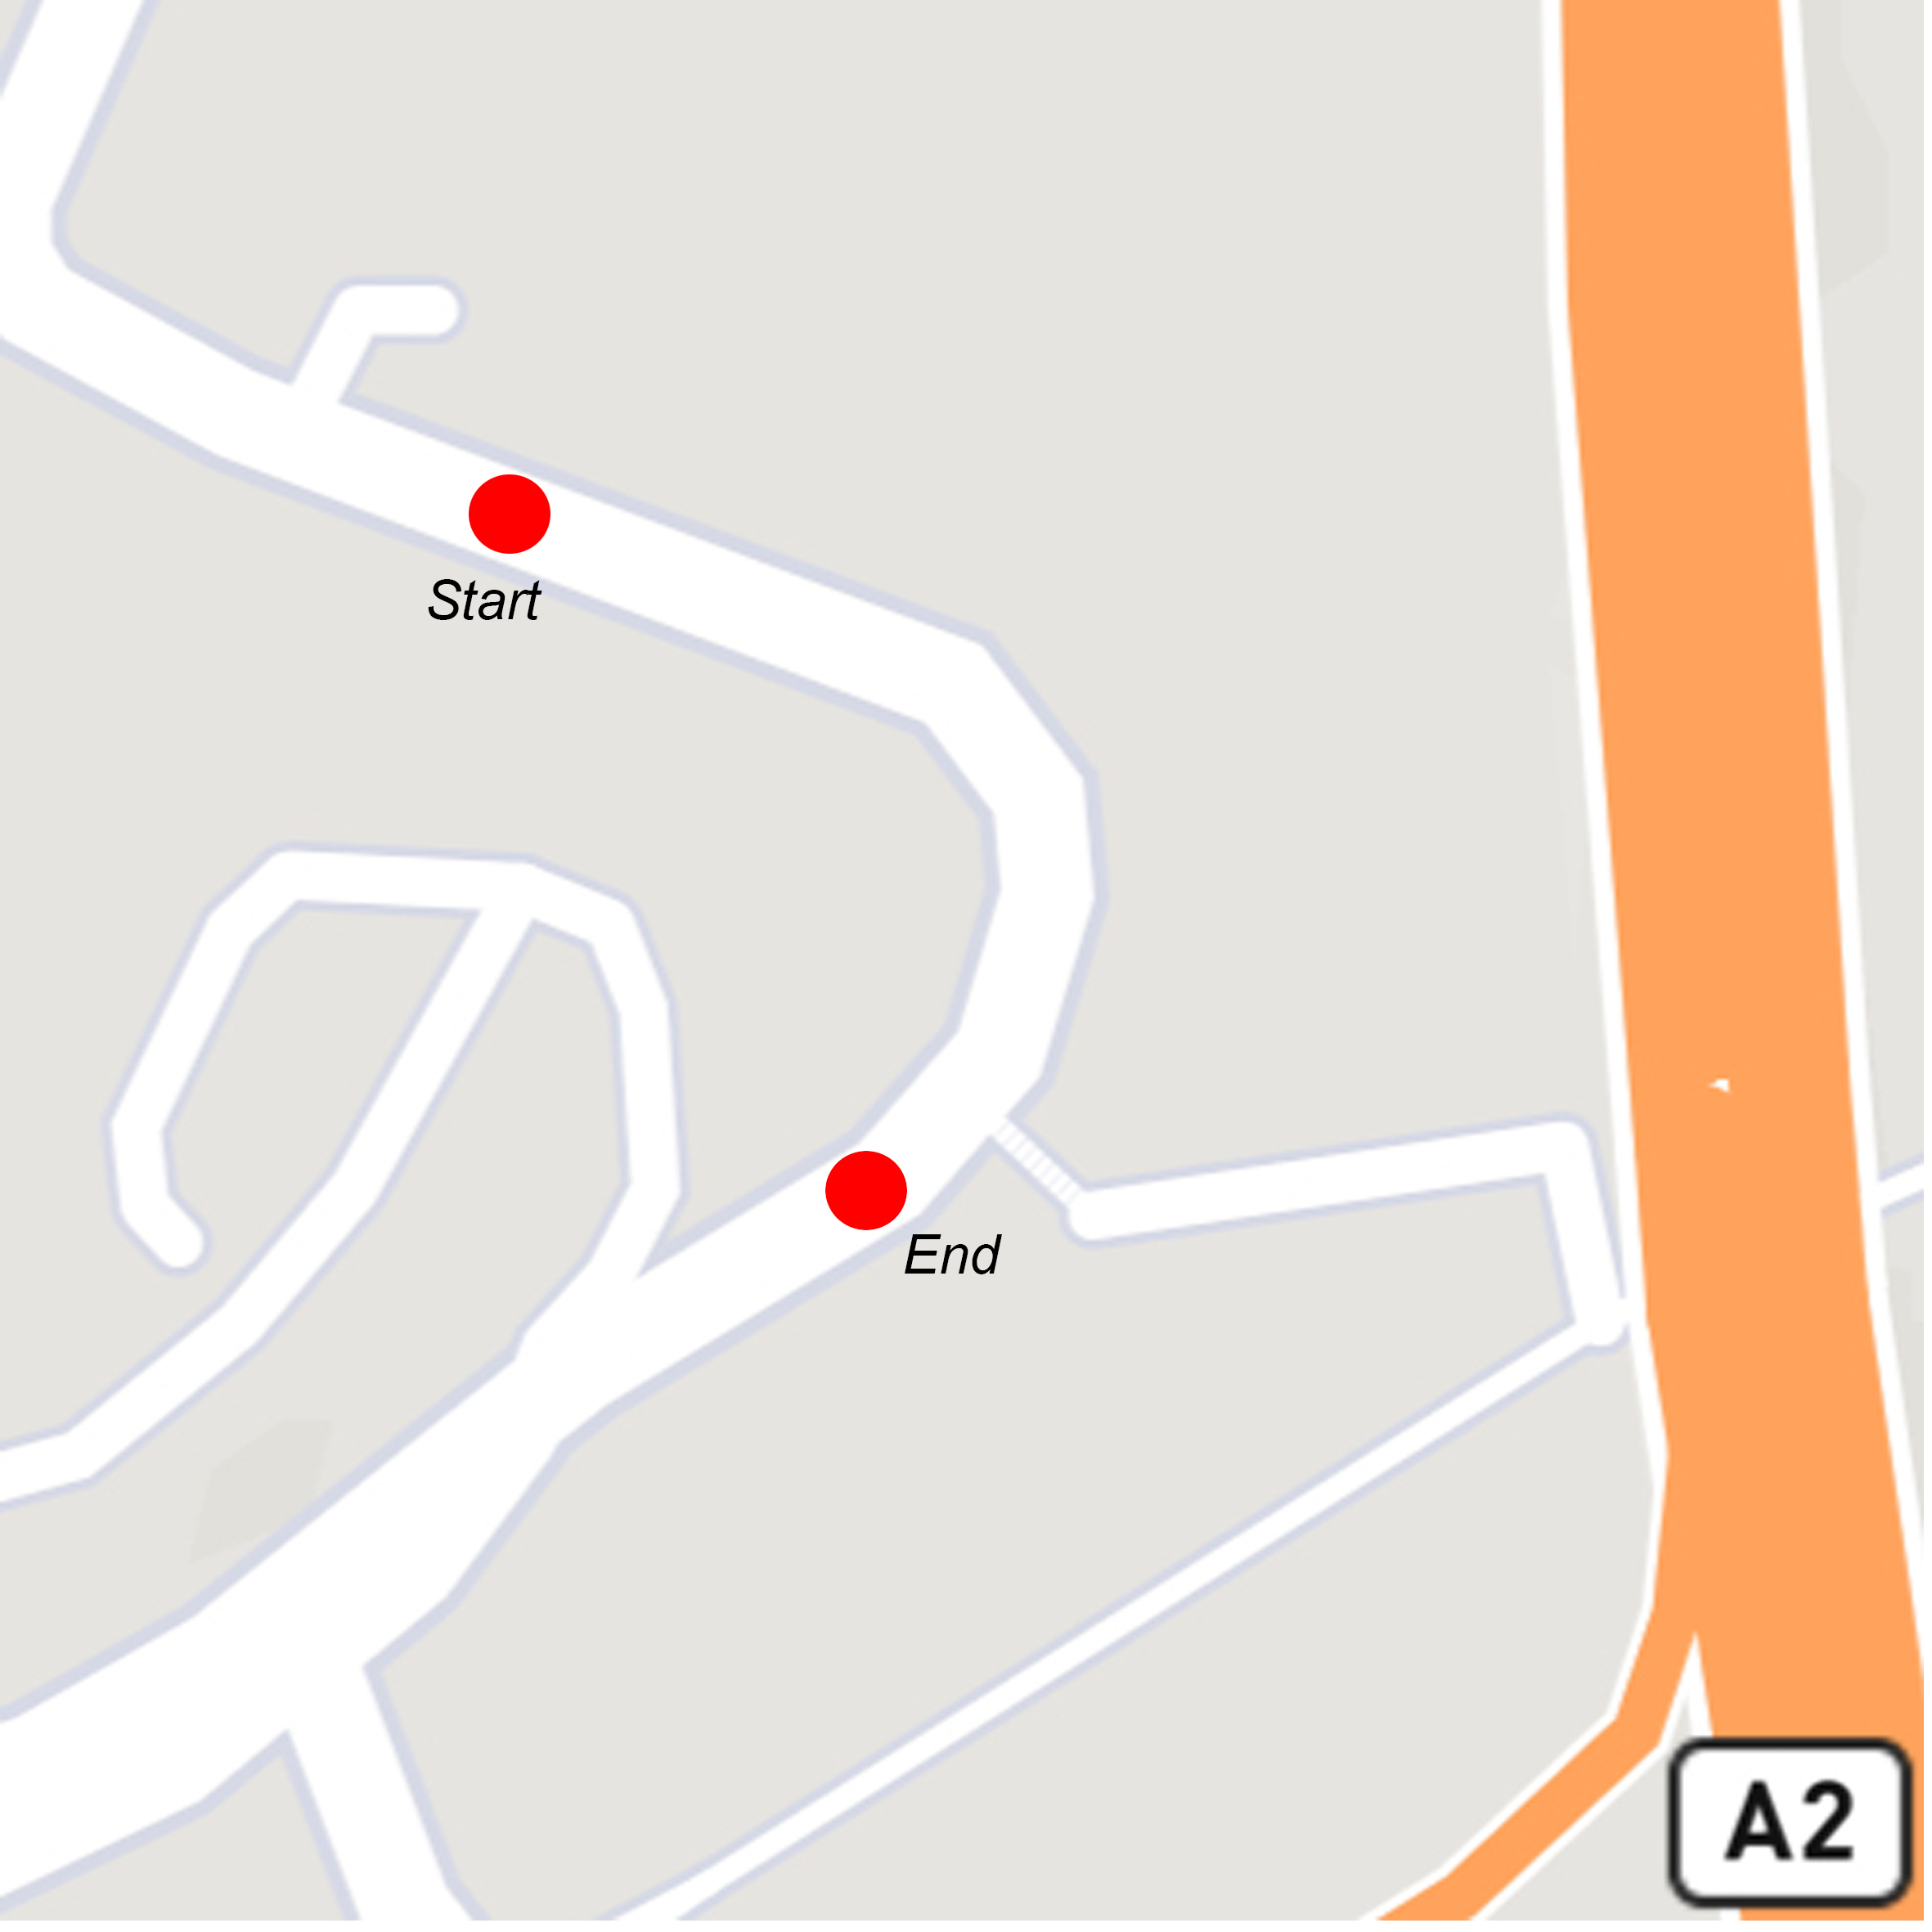
\includegraphics[scale=0.55]{Problem} \label{GPS Points Problem}
 \caption{Start and End points}
  \label{fig:GPS Points Problem}
\end{figure}


\noindent As we can see, we have two different GPS points, but we have a data accumulation at the $Start$ point, in our case equal to $100$ measurements and each of these has $Start$ point as GPS coordinate, the situation is analogue to the $End$ point.\\
Start point recordings refer to all $Start-End$ segment, but the intermediate coordinates of the segment are not recorded, and that is what is needed to properly locate the road surface conditions.\\
Therefore, a methodology has been developed, which from two different GPS points, allows determining the intermediate points in the segment. As shown in the code below.\\
\begin{pseudocode}{Redefine Latitude And Longitude}{Latitude[],Longitude[]}
\label{MergeSort}
\COMMENT{Create two collections of new Latitude and Longitude}\\
\BEGIN
NewLatitudeCollection[]\\
NewLongitudeCollection[]\\
index = 1\\ 
i = 1\\
\FOR y\GETS 2 \TO number \thinspace of \thinspace
Latitude \thinspace elements \DO \\
\BEGIN
FirstGPSCoordinate = Latitude[i], Longitude[i]\\
SecondGPSCoordinate = Latitude[y], Longitude[y]\\
\IF \CALL{distance} {FirstGPSCoordinate,SecondGPSCoordinate} \neq 0 \DO\\
\BEGIN
\COMMENT{distance function, use haversine formula, that is next explained}\\
NewLatitudeCollection [index] \GETS Latitude[i]\\
index++\\
NewLongitudeCollection[index] \GETS Longitude[i]\\
index++\\
latitudeDifference = \dfrac{Latitude[i]\quad minus \quad Latitude[y]}{y-i}\\\\
longitudeDifference = \dfrac{Longitude[i]\quad minus \quad Longitude[y]}{y-i}\\
\FOR k\GETS i+1 \TO y-1\DO \\
\BEGIN
NewLongitudeCollection[index]=NewLongitudeCollection[index-1] + longitudeDifference\\
index++\\
NewLatitudeCollection[index]=NewLatitudeCollection[index-1] + latitudeDifference\\
index++\\
\END \\

NewLatitudeCollection [index] \GETS Latitude[y]\\
index++\\
NewLongitudeCollection[index] \GETS Longitude[y]\\
index++\\
i \GETS y\\ 
\END
\END
\END
\end{pseudocode} 	



The proposed algorithm, when distinguishing two points having a distance between them different from $0$ $\si{\km}$, calculated by the \textit{haversine formula} that will be explained later, begins the definition of intermediate GPS points in the segment.\\
Beginning from the $Start$ point, until to the $End$ point, all intermediate points for both Latitude and Longitude will be calculated, as the previous point plus the difference in Latitude between the Start point and the End point, divided by the number of occurrences between Start and End, analogue procedure for Longitude.\\\\
Final result is shown in the figure:

\vspace{0.15cm}
\begin{figure}[H]	
\centering
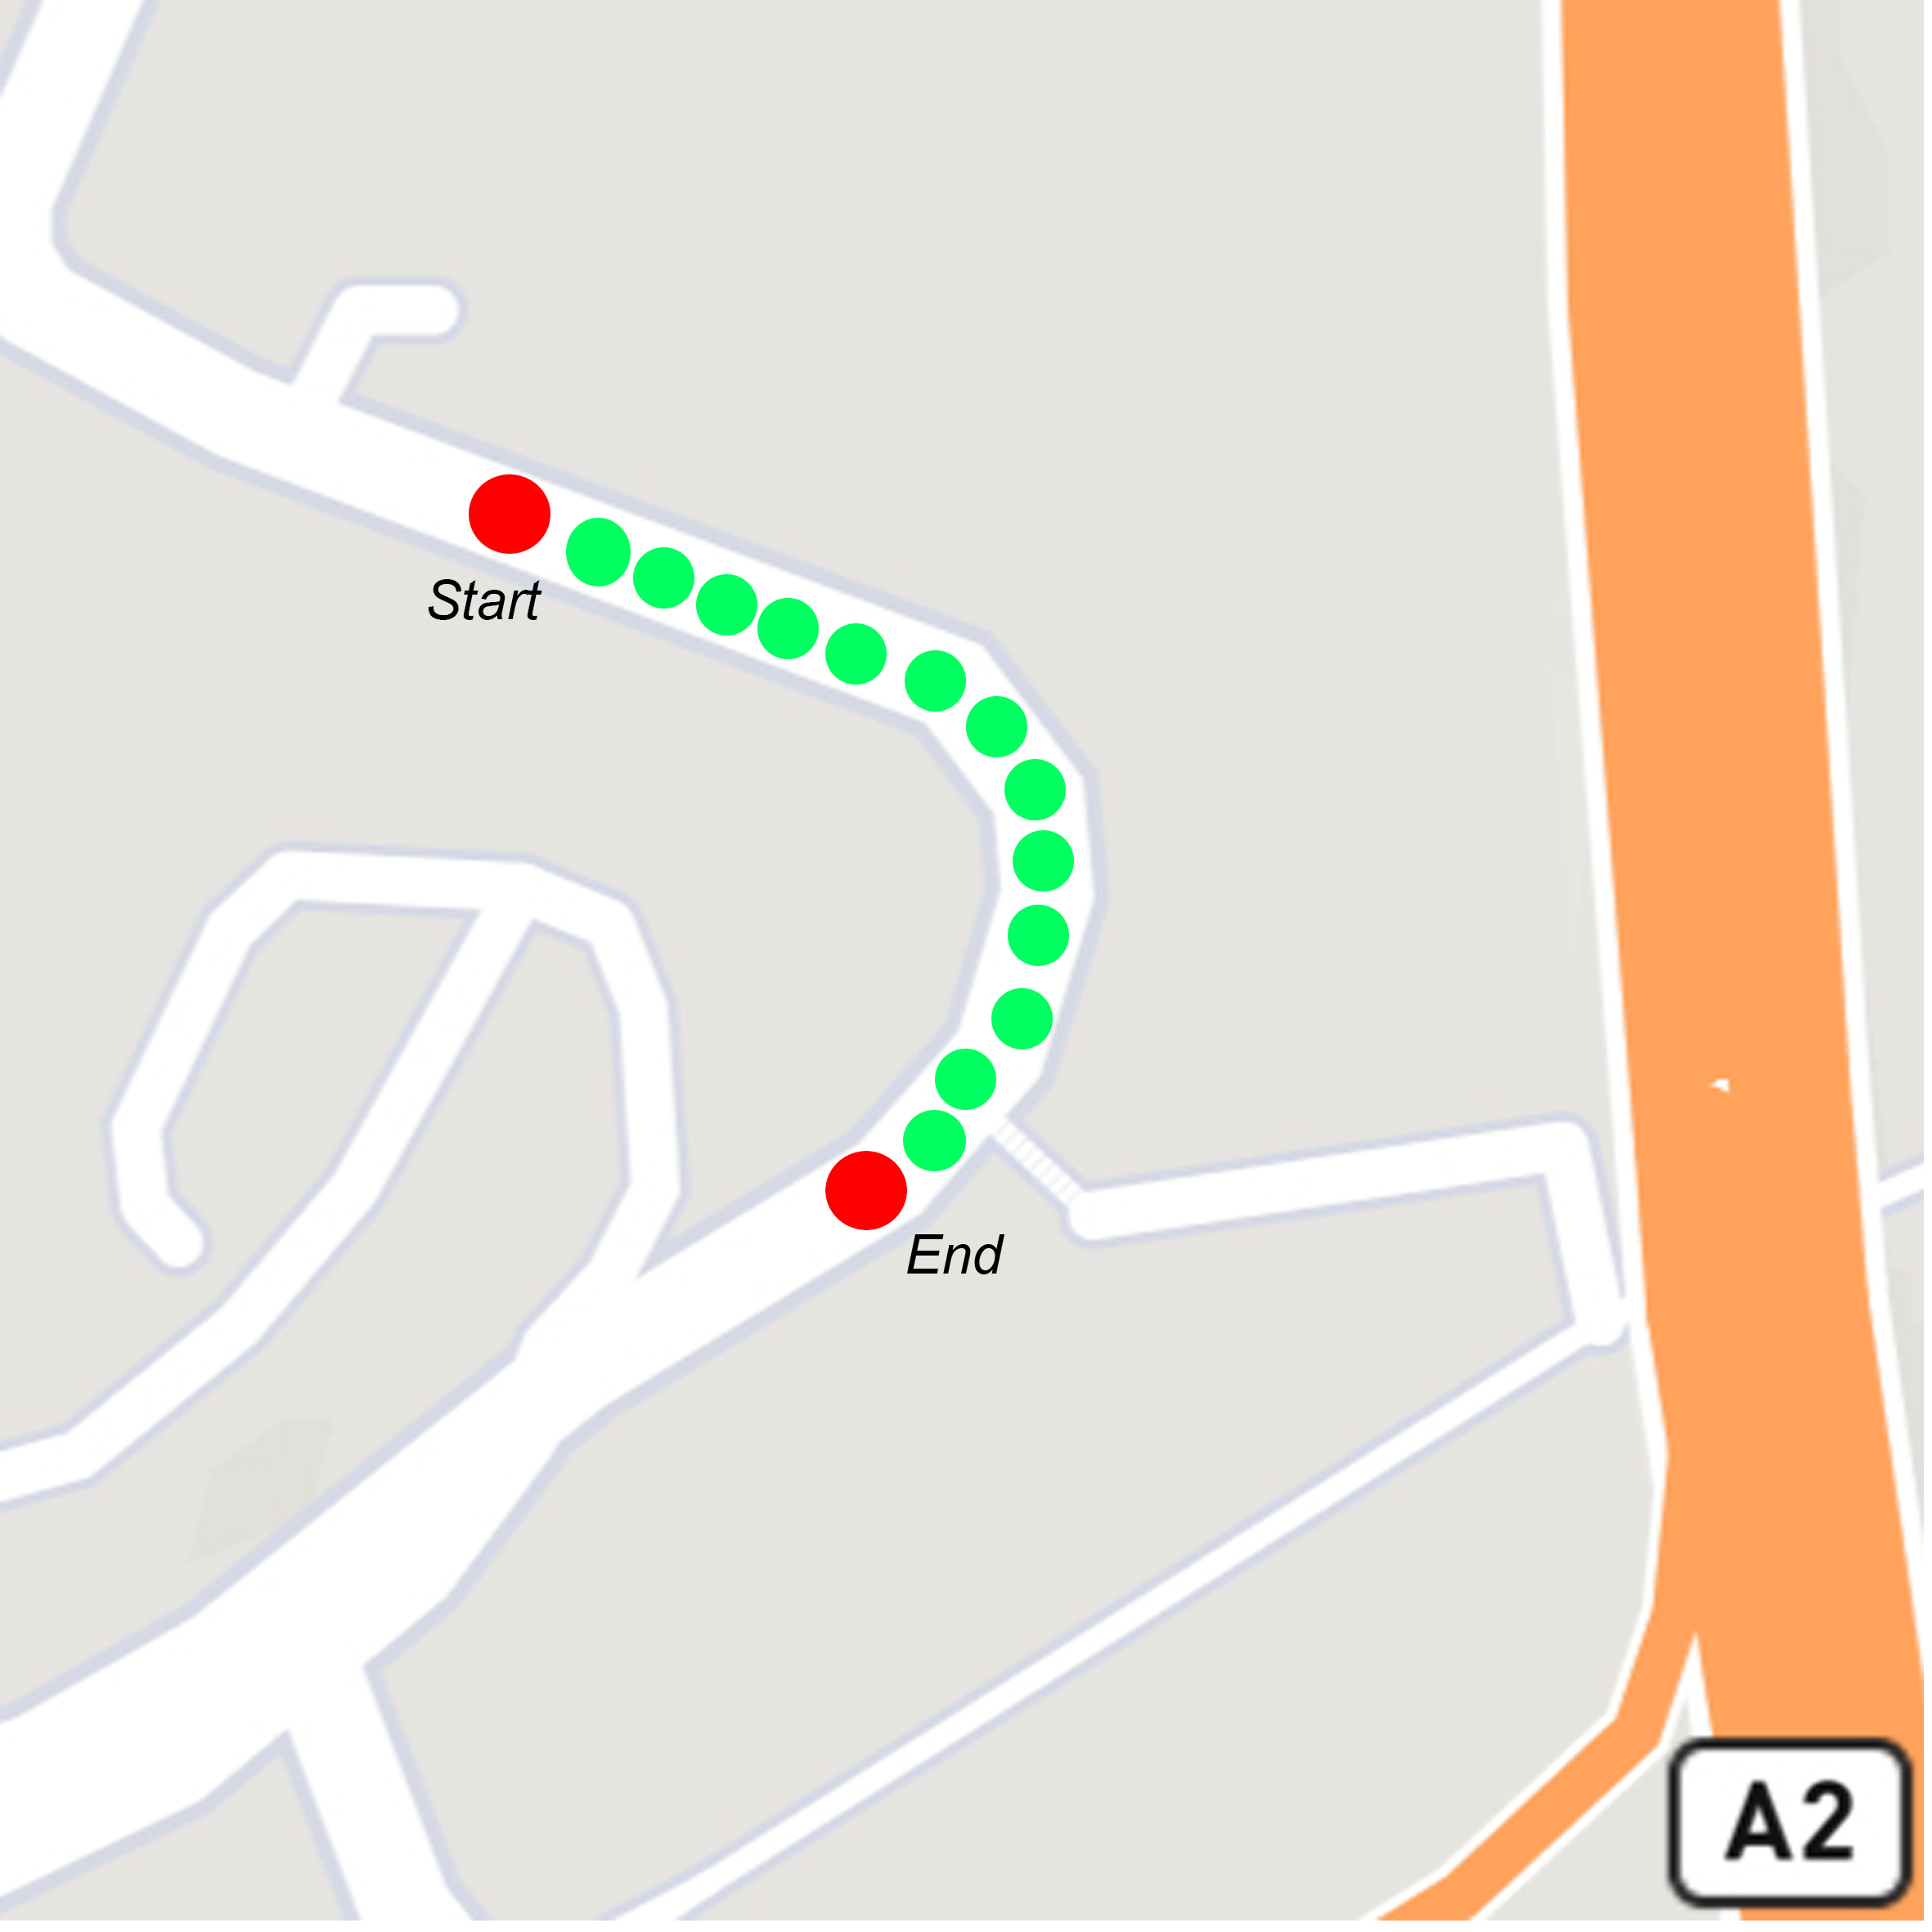
\includegraphics[scale=0.55]{ProblemSolved} \label{Solved GPS Points Problem}
 \caption{Start and End points}
  \label{fig:Solved GPS Points Problem}
\end{figure}


\end{document}


